% !TeX root = thesis.tex
%--------------------------------------------------------------------%
%
% Template TA LaTeX Teknik Informatika ITERA.
% Editor: Radhinka Bagaskara, Martin C.T. Manullang, iwawiwi
% Version 2025.3
%
% Berdasarkan:
% 1. Template Microsoft Word Tugas Akhir Informatika ITERA
% https://drive.google.com/file/d/1ZGk0GzCovn7iPYFXfmmWPUmS1PqBW1Ml/view
% 2. "Templat LaTeX Tesis Informatika ITB" oleh Petra Barus & Peb Ruswono Aryan
% https://github.com/petrabarus/if-itb-latex
%--------------------------------------------------------------------%
%
% Berkas ini berisi struktur utama dokumen LaTeX.
%
%--------------------------------------------------------------------%

% Set jenis dokumen Tugas Akhir
\documentclass[11pt, onecolumn, twoside, final]{report}

\input{config/config.sty}

\bibliography{references}

\begin{document}
% 	\pagestyle{plain}
% 	\fancyhf{}
% 	\rfoot{Halaman \thepage}%

    %----------------------------------------------------------------%
    % Konfigurasi Informasi Tugas Akhir
    %----------------------------------------------------------------%
    
    % Judul Tugas Akhir
    \title{IDENTIFIKASI PENYAKIT PADA DAUN BIBIT KELAPA SAWIT DENGAN PENDEKATAN NAÏVE BAYES MENGGUNAKAN OPTIMASI GENETIC ALGORITHM DAN PARTICLE SWARM OPTIMIZATION\\[0.2cm]{\normalfont\normalsize(Studi Kasus: PT Perkebunan Nusantara IV Regional 7 Kebun Bekri)}}      % Judul Tugas Akhir dalam Bahasa Indonesia 	
% DITULIS DALAM HURUF KAPITAL; Font size 16 pt; Bold; Tidak melebihi 4 baris
    \titleEN{IDENTIFICATION OF DISEASES IN OIL PALM SEEDLING LEAVES USING A NAÏVE BAYES CLASSIFIER OPTIMIZED BY GENETIC ALGORITHM AND PARTICLE SWARM OPTIMIZATION\\[0.2cm]{\normalfont\normalsize(Case Study: PT Perkebunan Nusantara IV Regional 7 Kebun Bekri)}}      % Judul Tugas Akhir dalam Bahasa Inggris
    
    % Informasi Mahasiswa
    \author{Natasya Ate Malem Bangun}		% Nama Mahasiswa
	\nim{121140052}			% NIM Mahasiswa
	
	%Informasi Dosen Pembimbing
	\dosbingA%
		{Meida Cahyo Untoro, S.Kom., M.Kom.}%	% Nama Dosen Pembimbing 1
		{NIP. 19890518 201903 1 011}				% NIP Dosen Pembimbing 1
	\dosbingB%
		{Nama dan Gelar Pembimbing II}%	% Nama Dosen Pembimbing 2
		{NIP. 123456789}				% NIP Dosen Pembimbing 2
		
	%Informasi Dosen Penguji
	\pengujiA%
		{Martin Clinton Tosima Manullang, Ph.D.}%	% Nama Dosen Penguji 1
		{NIP. 199301092019031017}				% NIP Dosen Penguji 1
	\pengujiB%
		{Andika Setiawan, S.Kom., M.Cs.}%	% Nama Dosen Penguji 2
		{NIP. 199111272022031007}				% NIP Dosen Penguji 2

	\sloppy % mencegah text overflow. (Jose)

    % --- Cover tanpa nomor ---
    \pagenumbering{gobble} % cover: nomor halaman tidak dicetak
    \input{chapters/cover-hard}

    % --- Mulai penomoran romawi ---
    \clearpage
    \pagenumbering{roman}
    \setcounter{page}{2}    % approval = ii (genap → kiri atas)

    % ATUR PENOMORAN AWAL (ii, iii, iv) - TANPA bolak-balik
    \fancyhf{} % Clear semua
    \renewcommand{\headrulewidth}{0pt}
    \fancyhead[R]{\thepage} % SEMUA halaman di kanan
    \pagestyle{fancy}

    \clearpage
\phantomsection% 
\addcontentsline{toc}{chapter}{Lembar Pengesahan}


% \begin{center}

% 	\large \bfseries \MakeUppercase{Lembar Pengesahan}
    
%     \normalsize \normalfont \onehalfspacing \justify{
%     Tugas Akhir Sarjana dengan judul Tugas Akhir Sarjana dengan judul "IDENTIFIKASI PENYAKIT PADA DAUN BIBIT KELAPA SAWIT DENGAN PENDEKATAN NAÏVE BAYES MENGGUNAKAN OPTIMASI GENETIC ALGORITHM DAN PARTICLE SWARM OPTIMIZATION (Studi Kasus: PT Perkebunan Nusantara IV Regional 7 Kebun Bekri)"  adalah benar dibuat oleh saya sendiri dan belum pernah dibuat dan diserahkan sebelumnya, baik sebagian ataupun seluruhnya, baik oleh saya ataupun orang lain, baik di Institut Teknologi Sumatera maupun di institusi pendidikan lainnya.}

% 	% Informasi Mahasiswa
% 	\setlength{\tabcolsep}{0pt}
% 	\begin{tabular}{p{0.7\textwidth} p{0.3\textwidth}}
% 		Lampung Selatan, 21-05-2025 & %
% 		\multirow{6}{*}{
% 			% Kotak pasfoto 3x4
% 			\phantom{---} % Amazing hack biar kotaknya ke kanan (RDB)
% 			\begin{tikzpicture}
% 				\draw rectangle (3cm,4cm) node[pos=0.5] {Foto 3x4};
% 			\end{tikzpicture}
% 		}\\
% 		Penulis, \\
% 		& \\
% 		& \\
% 		& \\
% 		& \\
% 		\theauthor\\
% 		NIM \printnim
% 	\end{tabular}

% 	% Informasi Dosen
% 	\centering Diperiksa dan disetujui oleh,
% 	\justify
%     \setlength{\tabcolsep}{0pt}
%     \begin{tabular}{ m{0.5cm}  m{0.7\textwidth} >{\centering\arraybackslash}m{0.3\textwidth}}
%         \multicolumn{2}{c}{Pembimbing} & \multicolumn{1}{c}{Tanda Tangan} \\
% 		1. & \printnamadosbinga & \\
% 		 & \printnipdosbinga & ......................\\
% 		% 2. & \printnamadosbingb & \\
% 		%  & \printnipdosbingb & ......................\\
% 		& \\[0.25cm]
% 		%  & \\
% 		\multicolumn{2}{c}{Penguji} & \multicolumn{1}{c}{Tanda Tangan} \\
% 		1. & \printnamapengujia & \\
% 		& \printnippengujia & ......................\\
% 		2. & \printnamapengujib & \\
% 		& \printnippengujib & ......................\\
%     \end{tabular}
% %	\vfill

% 	\begin{center}
% 		\fontsize{10pt}{12pt}
% 		Disahkan oleh,\\
% 		Koordinator Program Studi Teknik Informatika\\
% 		Fakultas Teknologi Industri\\
% 		Institut Teknologi Sumatera
% 		\vspace{2cm}\\
% 		Andika Setiawan, S.Kom., M.Cs. \\ % TODO: make automatic
% 		NIP 19911127 2022 03 1 007 \\
% 	\end{center}
% 	\vfill

% \end{center}
% \clearpage


\clearpage
\pagestyle{fancy}
\fancyhf{}
\fancyhead[R]{\thepage}
\phantomsection% 
\addcontentsline{toc}{chapter}{LEMBAR PENGESAHAN}

\begin{center}

	\large \bfseries \MakeUppercase{Lembar Pengesahan}
    
    \small \normalfont \singlespacing \justify{
    Tugas Akhir Sarjana dengan judul 
	"IDENTIFIKASI PENYAKIT PADA DAUN BIBIT KELAPA SAWIT DENGAN PENDEKATAN NAÏVE BAYES MENGGUNAKAN OPTIMASI GENETIC ALGORITHM DAN PARTICLE SWARM OPTIMIZATION (Studi Kasus: PT Perkebunan Nusantara IV Regional 7 Kebun Bekri)" adalah benar dibuat oleh saya sendiri dan belum pernah dibuat dan diserahkan sebelumnya, baik sebagian ataupun seluruhnya, baik oleh saya ataupun orang lain, baik di Institut Teknologi Sumatera maupun di institusi pendidikan lainnya.}
	\vspace{0.1cm}
    %Dengan ini saya menyatakan bahwa Tugas Akhir Sarjana berjudul "{\thetitle}" adalah karya orisinal saya. Tugas akhir ini belum pernah diserahkan atau diterbitkan sebelumnya, baik sebagian maupun seluruhnya, oleh saya atau pihak lain, di Institut Teknologi Sumatera maupun institusi pendidikan lainnya.
    %Saya menyatakan bahwa Tugas Akhir berjudul "{\thetitle}" merupakan hasil karya saya sendiri dan belum pernah diajukan, baik sebagian maupun seluruhnya, di Institut Teknologi Sumatera atau institusi pendidikan lain oleh saya maupun pihak lain.

	% Informasi Mahasiswa
	\setlength{\tabcolsep}{0pt}
	\begin{tabular}{p{0.59\textwidth} p{0.3\textwidth}}
        \vspace{0.1cm}
		Lampung Selatan, 21 Mei 2025 & %
		\multirow{6}{*}{
			% Kotak pasfoto 3x4
			\phantom{---} % Amazing hack biar kotaknya ke kanan (RDB)
			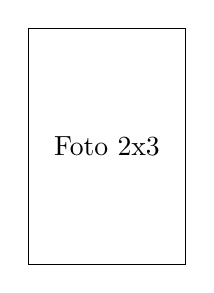
\begin{tikzpicture}
				\draw rectangle (2cm,3cm) node[pos=0.5] {Foto 2x3};
			\end{tikzpicture}
		}\\
		Penulis, \\
		& \\
		& \\
		%& \\
		\theauthor\\
		NIM \printnim
	\end{tabular}
	% Informasi Dosen
	\vspace{0.3cm}
        \begin{center}
        Diperiksa dan disetujui oleh,
        \end{center}
        \vspace{0.3cm}

	\justify
    \setlength{\tabcolsep}{0pt}
    \begin{tabular}{ m{0.5cm}  m{0.7\textwidth} >{\centering\arraybackslash}m{0.3\textwidth}}
        \multicolumn{2}{c}{\hspace*{-50pt}Pembimbing} & \multicolumn{1}{c}{Tanda Tangan} \\[2pt]
		1. & \printnamadosbinga & \\
		 & \printnipdosbinga & ............. \\[4pt]
		 %& \\
		\multicolumn{2}{c}{\hspace*{-70pt}Penguji} & \multicolumn{1}{c}{Tanda Tangan} \\[2pt]
		1. & \printnamapengujia & \\
		& \printnippengujia & ............. \\[4pt]
            %& \\
		2. & \printnamapengujib & \\
		& \printnippengujib & ............. \\
    \end{tabular}
%	\vfill

	\begin{center}
		\fontsize{10pt}{10pt}
        \vspace{0.35cm}
		Disahkan oleh,\\
		Koordinator Program Studi Teknik Informatika\\
		Fakultas Teknologi Industri\\
		Institut Teknologi Sumatera
		\vspace{1cm}\\
		Andika Setiawan, S.Kom., M.Cs. \\ % TODO: make automatic
		NIP 19911127 2022 03 1 007 \\
	\end{center}
	\vfill

\end{center}
\clearpage % Lembar Pengesahan (ii)
    \input{chapters/statement} % Halaman Pernyataan Orisinalitas (iii)
    \input{chapters/publication} % Halaman Persetujuan Publikasi (iv)

    % MULAI BOLAK-BALIK DARI KATA PENGANTAR (v)
\clearpage
    \fancyhf{} % Clear semua
    \renewcommand{\headrulewidth}{0pt}
    \fancyhead[RO]{\thepage} % ganjil → kanan atas
    \fancyhead[LE]{\thepage} % genap → kiri atas
    \pagestyle{fancy}

    \clearpage
\phantomsection% 
\addcontentsline{toc}{chapter}{Kata Pengantar}
\thispagestyle{fancy}

\begin{justifying}
	\large \bfseries \centering \MakeUppercase{Kata Pengantar}
	\par
	\normalsize \normalfont \justifying
	
	Segala puji dan syukur kepada Tuhan Yesus Kristus yang merupakan sumber hikmat dan pengharapan sejati, atas kasih karunia-Nya yang senantiasa menyertai setiap langkah penulis hingga akhirnya dapat menyelesaikan Tugas Akhir berjudul “Identifikasi Penyakit pada Daun Bibit Kelapa Sawit dengan Pendekatan \textit{Naïve Bayes} Menggunakan Optimasi \textit{Genetic Algorithm} dan \textit{Particle Swarm Optimization}”. 
	Tugas Akhir ini bukan sekadar hasil dari kerja keras dan proses berpikir ilmiah, tetapi juga buah dari dukungan, doa, dan kehadiran banyak pihak yang secara langsung maupun tidak langsung telah memberikan kontribusi luar biasa. Oleh karena itu, dengan penuh hormat dan rasa terima kasih yang mendalam, penulis ingin menyampaikan apresiasi kepada:
	\begin{enumerate}[itemsep=1pt, topsep=0pt, parsep=0pt, partopsep=0pt]
		\item {Tuhan Yesus Kristus yang telah memberikan penulis kekuatan, kesehatan, dan hikmat dalam proses penyelesaian Tugas Akhir ini, tanpa kasih karunia-Nya, penulis tidak akan mampu menyelesaikannya ini.}
		\item {Ibu Sipta Purba dan Bapak Sempakata Bangun selaku Orang Tua  tercinta yang menjadi sumber kekuatan penulis dengan memberikan cinta kasih, dukungan, doa, dan harapan kepada penulis dalam menyelesaikan Tugas Akhir ini. Sehingga Tugas Akhir ini dapat terselesaikan dengan baik dan penulis persembahakan sebagai gelar yang akan disandang penulis.}
		\item {Pihak PT Perkebunan Nusantara IV Regional 7 Kebun Bekri, yang telah memberikan akses, izin, serta arahan selama pelaksanaan penelitian lapangan untuk Tugas Akhir ini dapat berjalan dengan lancar.}
		\item {Bapak Andika Setiawan, S.Kom., M.Cs., Koordinator Program Studi Teknik Informatika ITERA sekaligus Dosen Penguji 2, atas bimbingan, kritik yang membangun, dan kepercayaan yang diberikan hingga Tugas Akhir ini dapat terselesaikan. Penulis juga berterima kasih atas kesempatan yang diberikan untuk mengikuti Magang Prodi dan Laboran 2025 di Prodi Teknik Informatika.}
		\item {Bapak Meida Cahyo Untoro, S.Kom. M.Kom. selaku Koordinator TA dan Dosen Pembimbing yang telah memberikan masukan, saran dan kelancaran kepada penulis dalam menyelesaikan Tugas akhir ini.}
		\item {Bapak Martin Clinton Tosima Manullang, Ph.D. selaku Dosen Penguji 1, atas arahan, ilmu, serta kesempatan berharga yang diberikan dalam mempertajam kemampuan ilmiah, memperdalam diskusi, dan memperluas wawasan riset yang sangat memperkaya proses penyelesaian Tugas Akhir ini.}
		\item {Bapak Andre Febrianto, S.Kom., M.Eng., selaku Dosen Pembimbing Akademik (Dosen Wali) yang mendampingi penulis sejak awal perkuliahan hingga akhir studi, atas arahan dan dukungan yang sangat membantu penyelesaian studi di Program Studi Teknik Informatika ITERA.}
		\item {Rekan-rekan Capstone Project, yaitu Benedictus Budhi Dharmawan dan Tobyanto Putra Mandiri, atas kebersamaan, dukungan, dan pemikiran berharga yang senantiasa dibagikan sepanjang perjalanan ini, sehingga setiap tantangan terasa lebih ringan.}
		\item {Teman-teman kecil saya, yaitu Emmia Sindilosa Ginting, Chetrine br Milala, dan Brigita May Putri Rosari Sidabutar, yang hadir dalam suka dan duka. Terima kasih telah menjadi tempat berbagi cerita, bertumbuh bersama, dan menguatkan penulis hingga akhir masa studi dan proses penyelesaian Tugas Akhir ini.}
		\item {Rekan-rekan yang memberi warna, semangat, dan keceriaan selama perjalanan Tugas Akhir ini, yaitu Steganonegai Team (Alvin-Marchell-Attar), Event Pejuang TA (Alvin, Atha, Attar, Marchell, Nopri, Pandu, Tara, Qaessar, dan Vania), FamilyMart Team, Stoberi Salkomsel, Proyek Kelapa Sawit Team, Ruang TA Team, Permata GBKP Runggun Bandar Lampung, dan BOS Team. Terima kasih atas setiap tawa, dukungan, kebersamaan yang menjadi penguat luar biasa, kehadiran kalian benar-benar berarti bagi penulis.}
		\item {Bapak Radhinka Bagaskara, S.Si.Kom., M.Si., M.Sc., selaku Koordinator Laboratorium Teknik 3 dan pengelola Ruang TA, atas fasilitas dan suasana kerja yang kondusif yang diberikan kepada penulis dalam menyelesaikan riset ini, bahkan hingga larut malam. Ucapan terima kasih juga penulis sampaikan kepada Ibu Leslie Anggraini, S.Kom., M.Cs. dan Ibu Miranti Verdiana, M.Si., atas dukungan, semangat, serta perhatian tulus yang senantiasa diberikan selama masa studi penulis di Program Studi Teknik Informatika ITERA.}
		\item {Seluruh Dosen, Tenaga Pendidik, dan Staff Program Studi Teknik Informatika ITERA yang telah memberikan ilmu, inspirasi dan pengalaman selama perjalanan akademik penulis.}
		\item {Seluruh teman seperjuangan Teknik Informatika ITERA, khususnya Angkatan 2021 (Binary) atas kebersamaan dan dukungannya selama masa studi penulis.}
		\item {Diri penulis sendiri, atas dedikasi yang telah ditunjukkan selama proses perkuliahan hingga penyusunan Tugas Akhir, dan kesabaran dalam menghadapi berbagai tantangan yang muncul.}
		\item {Untuk seluruh pihak yang tidak dapat disebutkan satu per satu, terima kasih atas segala bentuk dukungan, baik langsung maupun tidak langsung yang telah menguatkan penulis selama menempuh studi dan menyelesaikan Tugas Akhir ini.}
	\end{enumerate} \par
	Akhir kata, penulis berharap semoga tugas akhir ini tidak hanya menjadi pencapaian pribadi, tetapi juga memberikan kontribusi nyata bagi pengembangan ilmu pengetahuan, khususnya dalam penerapan \textit{Machine Learning} untuk sektor pertanian di Indonesia. Amin.
	\vfill
	
\end{justifying}
\clearpage
 % Kata Pengantar (v)

    \clearpage
    \fancyhf{} % Clear semua
    \renewcommand{\headrulewidth}{0pt}
    \fancyhead[RO]{\thepage} % ganjil → kanan atas
    \fancyhead[LE]{\thepage} % genap → kiri atas
    \pagestyle{fancy}

    \clearpage
\phantomsection% 
\addcontentsline{toc}{chapter}{Ringkasan}
\thispagestyle{fancy}

\begin{center}
	\large \bfseries \MakeUppercase{Ringkasan}\\
	\begingroup
	\setstretch{1.0} 
	\normalsize \normalfont {\thetitle}\\
	\endgroup
	\normalsize \normalfont {\theauthor}\\
	\bigskip
	
	\normalsize \normalfont \justifying
	Kelapa sawit termasuk komoditas penting di Indonesia karena memberikan kontribusi ekonomi yang signifikan. Namun, dalam proses budidaya, tanaman ini rentan terhadap serangan penyakit yang dapat menghambat pertumbuhan dan menurunkan produktivitas, terutama pada fase pembibitan. Terdapat lima kategori utama penyakit yang sering menyerang daun bibit kelapa sawit, yaitu bercak daun, daun berkerut, daun mengulung, daun menguning, dan daun berputar. Saat ini, penanganan penyakit tersebut masih mengandalkan pendekatan manual melalui identifikasi gejala visual pada daun. Namun, metode ini memiliki beberapa keterbatasan, di antaranya membutuhkan waktu dan sumber daya manusia yang besar serta berpotensi menimbulkan kesalahan dalam diagnosis.  

	Berdasarkan permasalahan tersebut, dilakukan penelitian untuk mengidentifikasi penyakit pada daun bibit kelapa sawit menggunakan pendekatan ekstraksi fitur \textit{Gray Level Co-occurrence Matrix} (GLCM) yang kemudian diklasifikasikan dengan algoritma \textit{Machine Learning Naïve Bayes}. Penelitian ini bertujuan untuk membangun model klasifikasi yang efisien secara komputasi dan mampu mengenali lima kelas penyakit tersebut. Dataset yang digunakan berasal dari PT Perkebunan Nusantara IV Regional 7 Bekri dan mencakup lima kelas penyakit daun bibit kelapa sawit. Untuk meningkatkan performa model, diterapkan dua metode optimasi, yaitu \textit{Genetic Algorithm} dan \textit{Particle Swarm Optimization}, guna mencari konfigurasi parameter terbaik.

	Penelitian ini menggunakan total 340 citra dengan pembagian data latih sebesar 80\% dan data uji sebesar 20\%. Setelah fitur citra diekstraksi menggunakan GLCM, hasilnya digunakan sebagai input bagi algoritma \textit{Naïve Bayes}. Optimasi dilakukan untuk menemukan kombinasi parameter terbaik dengan memanfaatkan \textit{Genetic Algorithm} dan \textit{Particle Swarm Optimization}. Hasil pengujian menunjukkan bahwa model \textit{Naïve Bayes} yang dihasilkan memiliki akurasi validasi tertinggi sebesar 56\%. Selain itu, evaluasi menggunakan \textit{Confusion Matrix} menunjukkan bahwa nilai rata-rata \textit{precision, recall,} dan \textit{F1-score} berada pada kisaran 55\% hingga 56\% untuk seluruh kelas penyakit. Meskipun performa model ini masih tergolong rendah, pendekatan yang digunakan dapat menjadi dasar awal untuk pengembangan sistem klasifikasi penyakit daun kelapa sawit yang lebih canggih dan akurat di masa mendatang.
	\vfill
	
\end{center}
\clearpage % Ringkasan (vi)

    \fancyhf{} % Clear semua
    \renewcommand{\headrulewidth}{0pt}
    \fancyhead[R]{\thepage} % SEMUA halaman di kanan
    \pagestyle{fancy}

    \clearpage
\phantomsection% 
\addcontentsline{toc}{chapter}{Abstrak}
\thispagestyle{fancy}

\begin{center}
	\large \bfseries \MakeUppercase{Abstrak}\\
	\normalsize \normalfont {\thetitle}\\
	\normalsize \normalfont {\theauthor}\\
	\bigskip
	
	\normalsize \normalfont \justifying \singlespacing
	Tanaman kelapa sawit merupakan komoditas unggulan Indonesia yang memiliki peran penting dalam perekonomian nasional. Namun pada fase pertumbuhan, bibit kelapa sawit rentan terhadap  serangan berbagai penyakit, terutama pada daun yang dapat menurunkan kualitas dan produktivitas bibit. Oleh karena itu, deteksi dini terhadap penyakit berperan penting dalam menjamin kualitas bibit. Penelitian ini bertujuan untuk mengembangkan model klasifikasi penyakit pada daun bibit kelapa sawit berbasi pengolahan citra digital dan machine learning. Ekstraksi fitur tekstur dan nilai RGB dari daun dilakukan dengan metode Gray Level Co-occurrence Matrix (GLCM). Fitur tersebut kemudian diklasifikasi dengan algoritma Naïve Bayes yang dioptimasi dengan dua metode, yakni Genetic Algorithm (GA) dan Particle Swarm Optimization (PSO) untuk meningkatkan akurasi pelatihan dari model. Dataset yang digunakan mencakup 5 kelas penyakit. Hasil pengujian menunjukkan bahwa model terbaik menghasilkan akurasi sebesar 56\% dengan rata-rata nilai presisi, recall, dan f1-score berkisar antara 55\% hingga 56\%. Pendekatan ini menunjukkan efisiensi komputasi yang baik dan dapat dijadikan baseline dalam pengembangan model klasifikasi yang lebih akurat di masa mendatang.

	
	\textbf{Kata Kunci:  Identifikasi Penyakit, Kelapa Sawit, Naïve Bayes, Genetic Algorithm, Particle Swarm Optimization
}
	
	\vfill
	
\end{center}
\clearpage % Abstrak (Indonesia) (vii)
    \clearpage
\phantomsection% 
\addcontentsline{toc}{chapter}{Abstract}
\thispagestyle{fancy}

\begin{center}
	\large \bfseries \MakeUppercase{Abstract}\\
	\normalsize \normalfont {\thetitleEN}\\
	\normalsize \normalfont {\theauthor}\\
	\bigskip
	
	\normalsize \normalfont \justifying \singlespacing
	Palm oil is a leading commodity in Indonesia with a significant role in the national economy. However, during the growth phase, palm oil seedlings are vulnerable to various diseases, particulary on the leaves, which can reduce seedling quality and productivity. Therefore, early detection of leaf diseases is essential to ensure seedling quality. This study aims to develop a classification model for leaf diseases detection in palm oil seedlings based on digital image processing and machine learning. Texture and RGB features were extracted using the Gray Level Co-occurremce Matrix (GLCM) method. Theses features were then classified using the Naïve Bayes algorithm, optimized with 2 techniques: Genetic Algorithm (GA) and Particle Swarm Optimization (PSO), to improve the model's training accuracy. The dataset used includes 5 classes of diseases. Experimental results show that the best model achieved an accuracy of 56\%, with average precision, recall, and f1-score values ranging from 55\% to 56\%. This approach demonstrates good computational efficiency and can serve as a baseline for the development of more accurate classification models in the future.
	
	\textbf{Keywords: Disease Identification, Palm oil, Naive Bayes, Genetic Algorithm, Particle Swarm Optimization}
	
	\vfill
	
\end{center}
\clearpage % Abstrak (Inggris) (viii)

    % Daftar Isi (ix)
    \clearpage
    \fancypagestyle{plain}{%
    \fancyhf{}%
    \renewcommand{\headrulewidth}{0pt}%
    \fancyhead[R]{\thepage}% Nomor di kanan
    }

    \phantomsection
    \addcontentsline{toc}{chapter}{Daftar Isi}
    \fancyhf{}                   % Clear semua header/footer
    \renewcommand{\headrulewidth}{0pt}
    \fancyhead[RO]{\thepage}      % Semua halaman → nomor di kanan
    \fancyhead[LE]{\thepage}
    \pagestyle{fancy}
    \tableofcontents

    % Daftar Tabel (x)
    \clearpage
    \phantomsection
    \addcontentsline{toc}{chapter}{Daftar Tabel}
    \fancyhf{}
    \renewcommand{\headrulewidth}{0pt}
    \fancyhead[R]{\thepage}      % Semua halaman → nomor di kanan
    \pagestyle{fancy}
    \listoftables

    % Daftar Gambar (xi)
    \clearpage
    \phantomsection
    \addcontentsline{toc}{chapter}{Daftar Gambar}
    \fancyhf{}
    \renewcommand{\headrulewidth}{0pt}
    \fancyhead[RE]{\thepage}
    \fancyhead[LO]{\thepage}
    \pagestyle{fancy}
    \listoffigures

    % Daftar Persamaan (xii)
    \clearpage
    \phantomsection
    \addcontentsline{toc}{chapter}{Daftar Rumus}
    \fancyhf{}
    \renewcommand{\headrulewidth}{0pt}
    \fancyhead[RE]{\thepage}
    \fancyhead[LO]{\thepage}
    \listofmyequations
    %----------------------------------------------------------------%
    % Konfigurasi Bab - Mulai penomoran arabic
    %----------------------------------------------------------------%
    \clearpage
    \renewcommand{\chaptername}{BAB}
    \renewcommand{\thechapter}{\Roman{chapter}}
    \renewcommand\thesection{\arabic{chapter}.\arabic{section}}
    
    % Reset penomoran halaman menjadi arabic
    \setcounter{page}{1}
    \pagenumbering{arabic}
    
    % Atur penomoran arabic bolak-balik
    \fancyhf{} % Clear semua header dan footer
    \renewcommand{\headrulewidth}{0pt} % Hilangkan garis header
    \fancyhead[RO]{\thepage} % Halaman ganjil: kanan atas
    \fancyhead[LE]{\thepage} % Halaman genap: kiri atas
    
    % Setting khusus untuk halaman pertama chapter (nomor di tengah bawah)
    \fancypagestyle{plain}{%
        \fancyhf{}%
        \renewcommand{\headrulewidth}{0pt}
        \fancyfoot[C]{\thepage} % Nomor halaman di tengah bawah
    }
    
    \pagestyle{fancy} % Terapkan style fancy untuk halaman biasa
    
    % Set spasi antar paragraf menjadi 0pt
    \setlength{\parskip}{0pt}
    
    %----------------------------------------------------------------%

    %----------------------------------------------------------------%
    % Daftar Bab
    % Untuk menambahkan daftar bab, buat berkas bab misalnya `chapter-6` di direktori `chapters`, dan masukkan ke sini.
    %----------------------------------------------------------------%
    \justifying
    \newpage
\chapter{Pendahuluan} \label{Bab I}

\section{Latar Belakang} \label{I.Latar Belakang}
Tanaman kelapa sawit (\textit{Elaeis Guineensis Jacq}) merupakan salah satu pilar utama komoditas perkebunan Indonesia yang terkenal menghasilkan minyak nabati dalam jumlah besar secara efisien dan ekonomis, baik untuk pasar domestik maupun internasional \cite{gaffar2024minyak}. Dengan kondisi iklim tropis Indonesia membuat lingkungan ideal bagi pertumbuhan kelapa sawit, membuat negara menjadi salah satu produsen minyak kelapa sawit di dunia  dengan sebagian besar produksi ditujukan untuk ekspor dan sisanya memenuhi kebutuhan dalam negeri \cite{saragih2022pengaruh}\cite{imaduddin2023analisa}.

Namun, dibalik potensinya yang besar, proses pembibitan dan budidaya kelapa sawit tetap menghadapi berbagai tantangan, khususnya pada fase awal pertumbuhan. Pada fase awal pertumbuhan bibit kelapa sawit, terutama dalam rentang usia 1 minggu hingga 3 bulan sangat rentan terhadap serangan penyakit daun \cite{syafrianda2024analisis}. Beberapa gejala umum yang sering muncul adalah daun menguning akibat infeksi jamur \textit {Ganoderma Boninense}, bercak-bercak akibat jamur \textit {Curvularia}, daun yang menggulung, berputar dan berkerut akibat serangan hama atau faktor genetik \cite{lisnawita2024peningkatan}\cite{harahap2024optimalisasi}\cite{napitupulu2022ta}\cite{marcelian2023identifikasi}. 

Penyakit-penyakit ini dapat memperlambat pertumbuhan, menghambat fotosintesis bahkan berdampak negatif terhadap kualitas bibit yang akan ditanam di lahan produksi \cite{marcelian2023identifikasi}. Oleh karena itu, deteksi dini terhadap penyakit pada bibit kelapa sawit sangat penting untuk memastikan pertumbuhan optimal dan kualitas bibit yang baik. Namun, proses identifikasi penyakit ini sering kali memerlukan keahlian khusus dan waktu yang cukup lama, sehingga diperlukan pendekatan yang lebih efisien dan akurat untuk mendeteksi penyakit pada bibit daun kelapa sawit \cite{pakiding2025implementasi}.

Salah satu lokasi yang mengalami tantangan tersebut adalah PT Perkebunan Nusantara (PTPN) IV Regional 7 Kebun Bekri di Provinsi Lampung menunjukkan bahwa serangan penyakit pada daun bibit kelapa sawit menjadi salah satu kendala signifikan yang mempengaruhi kualitas dan kuantitas bibit siap tanam. Keterlambatan penanganan penyakit dapat mengurangi persentase bibit layak tanam yang pada akhirnya mempengaruhi produktivitas lahan secara keseluruhan.

Untuk menjawab tantangan ini, penelitian bertujuan untuk mengidentifikasi penyakit pada bibit kelapa sawit menggunakan teknologi pengolahan citra dan pembelajaran mesin. Pengolahan citra digunakan untuk mengekstraksi fitur penting seperti warna (RGB), tekstur (\textit {Gray Level Co-Occurrence Matrix} atau GLCM) dan bentuk \cite{yunianto2021klasifikasi}.

Proses klasifikasi mengelompokkan objek berdasarkan fitur-fitur atau nilai atribut unik dari setiap objeknya. Pada proses ini, klasifikasi jenis penyakit pada daun kelapa sawit menerapkan pengolahan citra digital yang mengolah dan menganalisis sebuah citra dengan inputan data citra untuk menghasilkan informasi berupa citra. Penerapan pengolahan citra digital digunakan sebagai pembeda antara struktur bentuk, tekstur dan warna pada daun kelapa sawit yang sehat dan yang terserang penyakit, sekaligus menjadi dasar untuk parameter dalam penelitian \cite{elvira2021klasifikasi}. Daun kelapa sawit akan diteliti lebih lanjut dengan fitur tekstur \textit {Gray Level Co-Occurrence Matrix} (GLCM) untuk menemukan perbedaan pada struktur daun, kemudian hasilnya akan diekstraksi dengan metode RGB untuk mengidentifikasi terkait kondisi daun melalui perbedaan warnanya \cite{sukmanapeningkatan}.

Metode klasifikasi \textit{Naïve Bayes} telah menunjukkan potensi signifikan dalam berbagai penelitian terkait identifikasi berbasis citra \cite{afriansyah2024algoritma}. Misalnya, pada penelitian Septian sebelumnya menunjukkan bahwa metode klasifikasi seperti \textit{Naïve Bayes} mampu bekerja cukup baik dalam mengenali pola berdasarkan fitur visual dengan teknik \textit{10-Fold Cross Validation} yang berhasil mencapai akurasi hingga 86,06\% dalam membedakan jamur beracun dan tidak beracun \cite{prayoga2019implementasi}.

Lain halnya dengan penelitian oleh penelitian Ardi dkk yang menerapkan \textit{Naïve Bayes} untuk mendeteksi penyakit pada daun tanaman tomat berdasarkan fitur warna dan bentuk dengan GLCM dan \textit{Naïve Bayes} menunjukkan tingkat akurasi sebesar 80\% dari 15 dataset yang digunakan \cite{nainggolan2022identifikasi}. Sementara itu, pada penelitian Felicia membandingkan efektivitas \textit{Naïve Bayes} dengan KNN untuk mengidentifikasi jenis buah apel menggunakan fitur tekstur \textit{Local Binary Pattern (LBP)} dan warna HSV. Penelitian tersebut menunjukkan bahwa \textit{Naïve Bayes} memberikan akurasi lebih tinggi, berkisar 97\% dibandingkan metode \textit {K-Nearest Neighbor} (KKN) berkisar 82\% \cite{febriana2021perbandingan}.

Berdasarkan studi-studi tersebut \cite{prayoga2019implementasi}\cite{nainggolan2022identifikasi}\cite{febriana2021perbandingan}, metode \textit{Naïve Bayes} terbukti efektif untuk tugas klasifikasi yang melibatkan fitur warna dan tekstur dan mampu meminimalkan nilai \textit{error} pada dataset yang cukup besar. Namun, akurasi metode ini masih dapat ditingkatkan dengan pendekatan optimasi. Oleh karena itu, dalam penelitian ini, digunakan integrasi metode \textit{Naïve Bayes} dengan teknik optimasi seperti \textit{Genetic Algorithm (GA)} dan \textit{Particle Swarm Optimization (PSO)} untuk meningkatkan performa klasifikasi.

\textit{Genetic Algorithm} (GA) terinspirasi oleh proses evolusi biologis \cite{dwiputra2024perancangan}\cite{patmawatioptimalisasi}, sedangkan Teknik \textit{Particle Swarm Optimization} (PSO) terinspirasi oleh perilaku sosial burung dan ikan. Keduanya merupakan metode optimasi yang telah terbukti efektif dalam meningkatkan akurasi klasifikasi, sehingga diharapkan dapat meningkatkan akurasi deteksi penyakit pada bibit kelapa sawit.

Optimasi ini akan membantu dalam menyempurnakan parameter, seperti \textit{Prior Probability} dan \textit{Likelihood Estimation}, sehingga model dapat beradaptasi lebih baik terhadap variasi data \cite{ozsoy2020use}. Dalam evaluasi kinerja model digunakan juga metode \textit{Confusion Matrix} yang memungkinkan analisis lebih rinci terhadap \textit{presisi, recall}, dan akurasi hasil klasifikasi \cite{manurung2024implementasi}.

\section{Rumusan masalah} \label{I.Rumusan Masalah}
\indent Berdasarkan latar belakang yang telah dijelaskan diatas, maka rumusan masalah yang terkait, antara lain:
\begin{enumerate}[noitemsep]
	\item Bagaimana proses implementasi dan pengembangan model \textit{Naïve Bayes} dengan \textit{Particle Swarm Optimization} (PSO) dan \textit{Genetic Algorithm} (GA) dalam mengidentifikasi penyakit pada daun bibit kelapa sawit?
	\item Apakah model \textit{Naïve Bayes} dengan \textit{Particle Swarm Optimization} (PSO) dan \textit{Genetic Algorithm (GA)} terbukti efektif dalam mengidentifikasi penyakit pada daun bibit kelapa sawit?
	\item Faktor-faktor apa saja yang mempengaruhi kinerja model \textit{Naïve Bayes} dengan \textit{Particle Swarm Optimization} (PSO) dan \textit{Genetic Algorithm (GA)} dalam mengidentifikasi penyakit pada daun bibit kelapa sawit?
\end{enumerate}

\section{Tujuan} \label{I.Tujuan}
\indent Berdasarkan rumusan masalah di atas, maka tujuan penelitian ini, antara lain:
\begin{enumerate}[noitemsep]
	\item Mengembangkan dan mengimplementasikan model klasifikasi penyakit pada daun bibit kelapa sawit menggunakan algoritma \textit{Naïve Bayes} dengan \textit{Particle Swarm Optimization} (PSO) dan \textit{Genetic Algorithm} (GA).
	\item Mengevaluasi efektivitas model \textit{Naïve Bayes} dalam mengidentifikasi penyakit pada daun bibit kelapa sawit.
	\item Menganalisis pengaruh fitur-fitur penting yang memengaruhi kinerja model \textit{Naïve Bayes} dengan \textit{Particle Swarm Optimization} (PSO) dan \textit{Genetic Algorithm (GA)} dalam mengidentifikasi penyakit pada daun bibit kelapa sawit.
\end{enumerate}

\section{Batasan Masalah} \label{I.Batasan}
\indent Berdasarkan rumusan masalah diatas, diperlukan beberapa batasan masalah agar menghindari perluasan masalah, antara lain:
\begin{enumerate}[noitemsep]
	\item Penelitian ini hanya berfokus pada identifikasi penyakit pada daun bibit kelapa sawit menggunakan metode \textit{Naïve Bayes} dengan optimasi \textit{Particle Swarm Optimization} (PSO) dan \textit{Genetic Algorithm} (GA).
	\item Penelitian ini hanya menggunakan dataset citra daun bibit kelapa sawit yang diambil dari PT Perkebunan Nusantara IV Regional 7 Kebun Bekri.
	\item Penelitian ini hanya difokuskan pada identifikasi penyakit yang menyerang daun bibit kelapa sawit dalam rentang usia 1 minggu hingga 3 bulan.
	\item Data yang digunakan berupa citra digital daun kelapa sawit, dengan fitur utama yang dianalisis adalah warna (RGB) dan tekstur (\textit{Gray Level Co-Occurrence Matrix (GLCM)}).
	\item Model klasifikasi yang digunakan adalah \textit{Naïve Bayes} dengan menggunakan \textit{Particle Swarm Optimization} (PSO) dan \textit{Genetic Algorithm} (GA), tanpa membandingkan dengan algoritma klasifikasi lainnya.
\end{enumerate}

\section{Manfaat Penelitian} \label{I.Manfaat}
\indent Penelitian ini diharapkan dapat memberikan manfaat, antara lain:
\begin{enumerate}[noitemsep]
	\item Memudahkan petani perkebunan kelapa sawit dan pihak terkait dalam mengidentifikasi penyakit pada daun bibit kelapa sawit secara cepat dan akurat. 
	\item Memberikan wawasan dan kontribusi dalam pengembangan teknologi identifikasi penyakit pada daun bibit kelapa sawit menggunakan metode \textit{Naïve Bayes} dengan optimasi \textit{Particle Swarm Optimization} (PSO) dan \textit{Genetic Algorithm} (GA).
	\item Menyajikan evaluasi tentang kinerja metode \textit{Naïve Bayes} dengan optimasi \textit{Particle Swarm Optimization} (PSO) dan \textit{Genetic Algorithm} (GA) dalam klasifikasi penyakit pada daun bibit kelapa sawit.
	\item Menjadi salah satu pembuktian akurasi model \textit{Naïve Bayes} dengan optimasi \textit{Particle Swarm Optimization} (PSO) dan \textit{Genetic Algorithm} (GA) pada penyakit daun bibit kelapa sawit.
	\item Menjadi referensi bagi penelitian selanjutnya yang berkaitan dengan identifikasi penyakit pada tanaman menggunakan teknologi pengolahan citra dan pembelajaran mesin.
\end{enumerate}

\section{Sistematika Penulisan} \label{I.Sistematika}
Pada penulisan Tugas Akhir ini, penulis menyusun sistematika penulisan sebagai berikut:
\subsection{Bab I}
\indent Bab I Pendahuluan membahas mengenai latar belakang permasalahan, rumusan masalah, tujuan penelitian, batasan-batasan masalah penelitian, manfaat penelitian, dan sistematika penulisan.
\subsection{Bab II}
\indent Bab II Tinjauan Pustaka membahas mengenai kajian tinjauan pustaka yang menjelaskan tentang pengertian, teori, dan penelitian terdahulu yang berkaitan dengan penelitian ini.
\subsection{Bab III}
\indent Bab III Analisis dan Perancangan membahas mengenai metodologi penelitian yang menjelaskan tentang langkah-langkah yang dilakukan dalam penelitian ini, mulai dari alur penelitian, pengumpulan data, pengolahan data, hingga analisis hasil.
\subsection{Bab IV}
\indent Bab IV Hasil dan Pembahasan membahas menganai hasil dan pembahasan yang menjelaskan tentang hasil penelitian yang diperoleh dengan alur yang tertera. 
\subsection{Bab V}
\indent Bab V Kesimpulan dan Saran berisi tentang kesimpulan dan saran yang menjelaskan tentang kesimpulan dari penelitian yang dilakukan dan saran-saran untuk penelitian selanjutnya.

    \newpage
\chapter{Tinjauan Pustaka} \label{Bab II}

% ISIAN
\section{Tinjauan Pustaka} \label{II.Tinjauan}
Penelitian pada bidang klasifikasi citra berbasis \textit{Machine Learning} telah banyak dilakukan dalam berbagai objek. Namun, implementasi model klasifikasi penyakit secara spesifik pada daun bibit kelapa sawit masih tergolong terbatas, baik dari segi jumlah kajian maupun pendekatan optimasi yang digunakan. Meskipun demikian, terdapat beberapa studi sebelumnya yang menggunakan algoritma \textit{Naïve Bayes} dan pendekatan optimasi seperti \textit{Genetic Algorithm} (GA) dan \textit{Particle Swarm Optimization} (PSO) dengan objek dan fitur yang berbeda.

Salah satu penelitian yang relevan dilakukan oleh Septian dkk yang memanfaatkan metode \textit{Naïve Bayes} untuk mengklasifikasikan jenis jamur berdasarkan dataset yang terdiri dari 8124 citra. Proses pembelajaran yang digunakan adalah teknik validasi silang \textit{10-Fold Cross Validation} untuk membagi data latih dan uji. Penelitian ini menunjukkan bahwa metode \textit{Naïve Bayes} mampu mencapai akurasi sebesar 86,06\% dalam membedakan jamur yang layak konsumsi dan yang beracun. Hal ini menunjukkan bahwa algoritma ini memiliki fleksibilitas tinggi dalam menangani klasifikasi data visual pada objek biologis \cite{prayoga2019implementasi}.

Penelitian lain yang dilakukan oleh Ardi dkk yang menerapkan \textit{Naïve Bayes} untuk mendeteksi penyakit pada daun tanaman tomat berdasarkan fitur warna dan bentuk dengan menggunakan \textit{Gray Level Co-occurrence Matrix (GLCM)} . Penelitian ini menunjukkan bahwa metode \textit{Naïve Bayes} dapat digunakan untuk mengidentifikasi penyakit pada tanaman dengan akurasi yang cukup baik, meskipun dataset yang digunakan lebih kecil dibandingkan dengan penelitian sebelumnya. Dalam penelitian ini, akurasi yang diperoleh mencapai 80\% dari 15 dataset yang digunakan \cite{nainggolan2022identifikasi}.

Penelitian oleh Felicia dkk yang membandingkan performa metode \textit{Naïve Bayes} dengan \textit{K-Nearest Neighbor (KNN)} dalam mengidentifikasi jenis buah apel. Pada proses ekstraksi menggabungkan fitur tekstur dari \textit{Local Binary Pattern (LBP)} dan warna dari model HSV. Dataset terdiri dari 100 citra yang terbagi menjadi 80 data latih, 10 data uji, dan 10 data evaluasi. Hasilnya menunjukkan bahwa \textit{Naïve Bayes} memperoleh akurasi sebesar 97\%, lebih tinggi dibandingkan KNN yang mencapai 82\%, sehingga dapat dikatakan \textit{Naïve Bayes} tetap relevan dan kompetitif dalam domain klasifikasi citra berbasis fitur warna dan tekstur \cite{febriana2021perbandingan}.

Penelitian lainnya dilakukan Sherin dkk yang membuktikan bahwa optimasi \textit{Particle Swarm Optimization (PSO)} efektif digunakan dalam memprediksi hasil panen tanaman cabai rawit setan di Kota Pagar Alam dengan data yang digunakan mencakup curah hujan, jenis hama, jenis pupuk, dan luas lahan. Terbukti dengan mengintegrasikan metode \textit{Naïve Bayes} dan \textit{Particle Swarm Optimization (PSO)} yang menghasilkan akurasi \textit{Naïve Bayes} meningkat dari 75\% menjadi 92\% setelah dioptimasi dengan PSO \cite{junisthia2023integrasi}.

Penelitian lain dilakukan oleh Dadang dkk dengan menerapkan \textit{Naïve Bayes} untuk mengklasifikasikan 5 jenis bunga kantong semar berdasarkan citra digital menggunakan fitur warna RGB. Penelitian ini juga memanfaatkan teknik data augmentasi dan metode \textit{holdout} untuk validasi. Dari total 1750 data latih dan 350 data uji, metode \textit{Naïve Bayes} berhasil mencapai akurasi sebesar 97,06\%, menunjukkan bahwa algoritma ini efektif untuk klasifikasi citra tanaman langka sekalipun \cite{mulyana2022optimasi}.

Penelitian lainnya oleh Evy yang bertujuan meningkatkan akurasi metode \textit{Naïve Bayes} dalam klasifikasi jenis bakteri dengan menambahkan algoritma genetika. Data terdiri dari 336 atribut numerik, termasuk fitur-fitur seperti Mcg, gvh, Lip, dan alm. Hasil penelitian menunjukkan bahwa penggunaan algoritma genetika mampu memperbaiki konfigurasi dan pemodelan pada \textit{Naïve Bayes}, sehingga akurasi meningkat dari 80,93\% menjadi 81,19\% pada klasifikasi 8 kelas protein bakteri \cite{10.31294/swabumi.v9i2.11217}.

% TABEL
% Tabel dengan ukuran font yang sama dengan dokumen utama
% {\small
% \begin{longtable}{|>{\centering\arraybackslash}p{0.03\textwidth}|
% >{\raggedright\arraybackslash}p{0.15\textwidth}|
% >{\raggedright\arraybackslash}p{0.15\textwidth}|
% >{\raggedright\arraybackslash}p{0.15\textwidth}|
% >{\raggedright\arraybackslash}p{0.10\textwidth}|
% >{\raggedright\arraybackslash}p{0.10\textwidth}|
% >{\raggedright\arraybackslash}p{0.20\textwidth}|}  % kolom terakhir fleksibel
% \caption{Tinjauan Pustaka} \label{Table:2. Tinjauan Pustaka} \\
% \hline
% \textbf{No} & \textbf{Judul} & \textbf{Masalah} & \textbf{Metode} & \textbf{Data} & \textbf{Hasil} & \textbf{Perbandingan} \\
% \hline
% \endfirsthead

% \hline
% \textbf{No} & \textbf{Judul} & \textbf{Masalah} & \textbf{Metode} & \textbf{Data} & \textbf{Hasil} & \textbf{Perbandingan} \\
% \hline
% \endhead


% 1 & Implementasi Metode \textit{Naïve Bayes Classifier} untuk Identifikasi Jenis Jamur (Septian Arie Prayoga, Ismasari Nawangsih, Tri Ngudi Wiyatno) & Menentukan akurasi metode \textit{Naïve Bayes Classifier} dalam klasifikasi jamur konsumsi dan beracun serta perancangan aplikasinya & \textit{Naïve Bayes} dengan \textit{10-Fold Cross Validation} & Dataset 8124 citra jamur & Akurasi 86,06\% & Penelitian ini berbeda dengan Prayoga dkk. pada objek kajian, metode fitur, dan optimasi. Prayoga dkk. mengklasifikasi jenis jamur menggunakan \textit{Naïve Bayes} tanpa segmentasi atau fitur warna/tekstur, sedangkan penelitian ini fokus pada penyakit daun kelapa sawit dengan fitur warna RGB, tekstur GLCM, segmentasi K-Means, serta optimasi \textit{GA} dan \textit{PSO}. Hasilnya mencapai akurasi 59\% dengan \textit{precision, recall}, dan \textit{F1-score} 58–59\%.\\
% \hline

% 2 & Identifikasi Penyakit Tanaman Tomat Berdasarkan Citra Penyakit Menggunakan Metode GLCM dan \textit{Naïve Bayes Classifier} (Ardi Nainggolan dkk.) & Meng-\linebreak identifikasi penyakit tanaman tomat berdasarkan citra daun, buah, dan batang & GLCM (ekstraksi fitur) dan \textit{Naïve Bayes Classifier} (klasifikasi penyakit) & 15 citra uji dengan ukuran sampel 3x3 piksel (manual) & Akurasi 80\% & Perbedaan penelitian ini dengan Ardi dkk. terletak pada objek, dataset, dan metode. Ardi dkk. fokus pada penyakit daun tomat (15 citra) dengan GLCM dan \textit{Naïve Bayes}, akurasi 80\%. Penelitian ini mendeteksi penyakit daun kelapa sawit (5 kelas) dengan GLCM dan \textit{Naïve Bayes} yang dioptimasi \textit{GA} dan \textit{PSO}, akurasi 59\% dan \textit{precision, recall, F1-score} 58–59\%, menekankan optimasi dan dataset lebih kompleks.\\
% \hline

% 3 & Perbandingan Klasifikasi \textit{Naïve Bayes} dan KNN untuk Meng-\linebreak 	identifikasi Jenis Buah Apel dengan Ekstraksi Ciri LBP dan HSV (Felicia Febriana dkk.) & Mem-\linebreak bandingkan efektivitas klasifikasi \textit{Naïve Bayes} dan KNN menggunakan fitur warna dan tekstur pada lima jenis apel & Klasifikasi menggunakan \textit{Naïve Bayes} dan KNN, dengan ekstraksi ciri HSV dan LBP & 100 citra apel (80 data latih, 10 evaluasi, 10 uji) & Akurasi \textit{Naïve Bayes} (HSV), sebesar 97\%, KNN (HSV) sebesar 82\% & Perbedaan penelitian ini dengan Felicia Febriana dkk. (2021) terletak pada objek, metode, fitur, dan hasil. Penelitian Felicia Febriana dkk. fokus pada identifikasi jenis buah apel dengan \textit{Naïve Bayes} dan KNN menggunakan fitur LBP (tekstur) dan HSV (warna), mencapai akurasi 90–97\%. Penelitian ini fokus pada penyakit daun bibit kelapa sawit menggunakan \textit{Naïve Bayes} dengan fitur tekstur GLCM dan optimasi \textit{GA} serta \textit{PSO}, dengan akurasi tertinggi 59\% dan \textit{precision, recall, F1-score} rata-rata 58–59\%.\\
% \hline


% 4 & Integrasi \textit{Particle Swarm Optimization} dengan \textit{Naïve Bayes} untuk Prediksi Tanaman Cabai (Sherin Junisthia dkk.) & Meningkatkan akurasi prediksi panen cabai rawit dengan optimasi waktu dan parameter \textit{Naïve Bayes} & Kombinasi \textit{Naïve Bayes} dan PSO, dalam kerangka CRISP-DM & Data pertanian Kota Pagar Alam dengan 8 variabel fitur & Akurasi tanpa PSO sebesar 75\%, dengan PSO sebesar 92\% & Perbedaan penelitian ini dengan penelitian cabai rawit terletak pada objek, fitur, dan hasil. Penelitian cabai rawit menggunakan data numerik untuk prediksi hasil panen dengan \textit{Naïve Bayes} dioptimasi \textit{PSO}, meningkatkan akurasi dari 75\% menjadi 92\%. Penelitian ini mendeteksi penyakit daun bibit kelapa sawit berbasis citra dengan fitur tekstur GLCM, diklasifikasikan \textit{Naïve Bayes} yang dioptimasi \textit{GA} dan \textit{PSO}, dengan akurasi 59\% dan \textit{precision, recall, F1-score} 58–59\%.\\
% \hline

% 5 & Optimasi Klasifikasi Bunga Kantong Semar Menggunakan \textit{Naïve Bayes}, Data Augmentasi dan PSO (Dadang Iskandar Mulyana dkk.) & Klasifikasi lima jenis bunga kantong semar dengan akurasi tinggi melalui augmentasi data & \textit{Naïve Bayes} dengan pembagian data menggunakan metode \textit{Holdout} (80\%-20\%) & 2100 citra (1750 latih, 350 uji) & Akurasi pelatihan dan pengujian sebesar 97,60\% & Perbedaan penelitian ini dengan penelitian kantong semar terletak pada objek, fitur, optimasi, dan hasil. Penelitian kantong semar mengklasifikasi 5 jenis citra dengan fitur RGB dan \textit{ImageNet}, menggunakan \textit{Naïve Bayes} tanpa optimasi, mencapai akurasi 97,60\%. Penelitian ini mengklasifikasi 5 kelas penyakit daun kelapa sawit dengan fitur tekstur GLCM, \textit{Naïve Bayes} dioptimasi \textit{GA} dan \textit{PSO}, dengan akurasi 59\% dan \textit{precision, recall, F1-score} 58–59\%.\\
% \hline

% 6 & Peningkatan Algoritma \textit{Naïve Bayes} Menggunakan Algoritma Genetika pada Klasifikasi Bakteri (Evy Priyanti) & Mengatasi keterbatasan akurasi klasifikasi bakteri dengan optimasi parameter \textit{Naïve Bayes} & \textit{Naïve Bayes} dan \textit{Genetic Algorithm} untuk tuning parameter & 336 atribut numerik untuk 8 kelas protein bakteri & Akurasi awal sebesar 80,93\%, meningkat menjadi 81,19\% & Perbedaan penelitian ini dengan penelitian bakteri terletak pada objek, fitur, optimasi, dan hasil. Penelitian bakteri menggunakan data numerik dan \textit{Naïve Bayes} yang dioptimasi \textit{Genetic Algorithm}, meningkatkan akurasi dari 80,93\% menjadi 81,19\%. Penelitian ini mengklasifikasi penyakit daun kelapa sawit berbasis citra dengan fitur tekstur GLCM, \textit{Naïve Bayes} dioptimasi \textit{GA} dan \textit{PSO}, dengan akurasi 59\% serta \textit{precision, recall, F1-score} 58–59\%.\\
% \hline


% \end{longtable}
% }
{
\renewcommand{\arraystretch}{1.0}
\setlength{\tabcolsep}{3pt}
% Contoh: custom size 8pt
\fontsize{9pt}{10pt}\selectfont  % {ukuran font}{jarak baris}
\begin{longtable}{|>{\centering\arraybackslash}p{0.04\textwidth}|
                  >{\raggedright\arraybackslash}p{0.16\textwidth}|
                  >{\raggedright\arraybackslash}p{0.16\textwidth}|
                  >{\raggedright\arraybackslash}p{0.16\textwidth}|
                  >{\raggedright\arraybackslash}p{0.10\textwidth}|
                  >{\centering\arraybackslash}p{0.12\textwidth}|
                  >{\raggedright\arraybackslash}p{0.22\textwidth}|}

\caption{Tinjauan Pustaka} \label{Table:2. Tinjauan Pustaka} \\
\hline
\textbf{No} & \textbf{Judul} & \textbf{Masalah} & \textbf{Metode} & \textbf{Data} & \textbf{Hasil} & \textbf{Perbandingan} \\
\hline
\endfirsthead

\hline
\textbf{No} & \textbf{Judul} & \textbf{Masalah} & \textbf{Metode} & \textbf{Data} & \textbf{Hasil} & \textbf{Perbandingan} \\
\hline
\endhead

1 & Implementasi Metode \textit{Naïve Bayes Classifier} untuk Identifikasi Jenis Jamur (Septian Arie Prayoga, Ismasari Nawangsih, Tri Ngudi Wiyatno) & Menentukan akurasi metode \textit{Naïve Bayes Classifier} dalam klasifikasi jamur konsumsi dan beracun serta perancangan aplikasinya & \textit{Naïve Bayes} dengan \textit{10-Fold Cross Validation} & Dataset 8124 citra jamur & Akurasi 86,06\% & Penelitian ini berbeda dengan Prayoga dkk. pada objek kajian, metode fitur, dan optimasi. Prayoga dkk. mengklasifikasi jenis jamur menggunakan \textit{Naïve Bayes} tanpa segmentasi atau fitur warna/tekstur, sedangkan penelitian ini fokus pada penyakit daun kelapa sawit dengan fitur warna RGB, tekstur GLCM, segmentasi K-Means, serta optimasi \textit{GA} dan \textit{PSO}. Hasilnya mencapai akurasi 59\% dengan \textit{precision, recall}, dan \textit{F1-score} 58–59\%.\\
\hline

2 & Identifikasi Penyakit Tanaman Tomat Berdasarkan Citra Penyakit Menggunakan Metode GLCM dan \textit{Naïve Bayes Classifier} (Ardi Nainggolan dkk.) & Meng -identifikasi penyakit tanaman tomat berdasarkan citra daun, buah, dan batang & GLCM (ekstraksi fitur) dan \textit{Naïve Bayes Classifier} (klasifikasi penyakit) & 15 citra uji dengan ukuran sampel 3x3 piksel (manual) & Akurasi 80\% & Perbedaan penelitian ini dengan Ardi dkk. terletak pada objek, dataset, dan metode. Ardi dkk. fokus pada penyakit daun tomat (15 citra) dengan GLCM dan \textit{Naïve Bayes}, akurasi 80\%. Penelitian ini mendeteksi penyakit daun kelapa sawit (5 kelas) dengan GLCM dan \textit{Naïve Bayes} yang dioptimasi \textit{GA} dan \textit{PSO}, akurasi 59\% dan \textit{precision, recall, F1-score} 58–59\%, menekankan optimasi dan dataset lebih kompleks.\\
\hline

3 & Perbandingan Klasifikasi \textit{Naïve Bayes} dan KNN untuk Meng -identifikasi Jenis Buah Apel dengan Ekstraksi Ciri LBP dan HSV (Felicia Febriana dkk.) & Mem -bandingkan efektivitas klasifikasi \textit{Naïve Bayes} dan KNN menggunakan fitur warna dan tekstur pada lima jenis apel & Klasifikasi menggunakan \textit{Naïve Bayes} dan KNN, dengan ekstraksi ciri HSV dan LBP & 100 citra apel (80 data latih, 10 evaluasi, 10 uji) & Akurasi \textit{Naïve Bayes} (HSV), sebesar 97\%, KNN (HSV) sebesar 82\% & Perbedaan penelitian ini dengan Felicia Febriana dkk. (2021) terletak pada objek, metode, fitur, dan hasil. Penelitian Felicia Febriana dkk. fokus pada identifikasi jenis buah apel dengan \textit{Naïve Bayes} dan KNN menggunakan fitur LBP (tekstur) dan HSV (warna), mencapai akurasi 90–97\%. Penelitian ini fokus pada penyakit daun bibit kelapa sawit menggunakan \textit{Naïve Bayes} dengan fitur tekstur GLCM dan optimasi \textit{GA} serta \textit{PSO}, dengan akurasi tertinggi 59\% dan \textit{precision, recall, F1-score} rata-rata 58–59\%.\\
\hline

4 & Integrasi \textit{Particle Swarm Optimization} dengan \textit{Naïve Bayes} untuk Prediksi Tanaman Cabai (Sherin Junisthia dkk.) & Meningkatkan akurasi prediksi panen cabai rawit dengan optimasi waktu dan parameter \textit{Naïve Bayes} & Kombinasi \textit{Naïve Bayes} dan PSO, dalam kerangka CRISP-DM & Data pertanian Kota Pagar Alam dengan 8 variabel fitur & Akurasi tanpa PSO sebesar 75\%, dengan PSO sebesar 92\% & Perbedaan penelitian ini dengan penelitian cabai rawit terletak pada objek, fitur, dan hasil. Penelitian cabai rawit menggunakan data numerik untuk prediksi hasil panen dengan \textit{Naïve Bayes} dioptimasi \textit{PSO}, meningkatkan akurasi dari 75\% menjadi 92\%. Penelitian ini mendeteksi penyakit daun bibit kelapa sawit berbasis citra dengan fitur tekstur GLCM, diklasifikasikan \textit{Naïve Bayes} yang dioptimasi \textit{GA} dan \textit{PSO}, dengan akurasi 59\% dan \textit{precision, recall, F1-score} 58–59\%.\\
\hline

5 & Optimasi Klasifikasi Bunga Kantong Semar Menggunakan \textit{Naïve Bayes}, Data Augmentasi dan PSO (Dadang Iskandar Mulyana dkk.) & Klasifikasi lima jenis bunga kantong semar dengan akurasi tinggi melalui augmentasi data & \textit{Naïve Bayes} dengan pembagian data menggunakan metode \textit{Holdout} (80\%-20\%) & 2100 citra (1750 latih, 350 uji) & Akurasi pelatihan dan pengujian sebesar 97,60\% & Perbedaan penelitian ini dengan penelitian kantong semar terletak pada objek, fitur, optimasi, dan hasil. Penelitian kantong semar mengklasifikasi 5 jenis citra dengan fitur RGB dan \textit{ImageNet}, menggunakan \textit{Naïve Bayes} tanpa optimasi, mencapai akurasi 97,60\%. Penelitian ini mengklasifikasi 5 kelas penyakit daun kelapa sawit dengan fitur tekstur GLCM, \textit{Naïve Bayes} dioptimasi \textit{GA} dan \textit{PSO}, dengan akurasi 59\% dan \textit{precision, recall, F1-score} 58–59\%.\\
\hline

6 & Peningkatan Algoritma \textit{Naïve Bayes} Menggunakan Algoritma Genetika pada Klasifikasi Bakteri (Evy Priyanti) & Mengatasi keterbatasan akurasi klasifikasi bakteri dengan optimasi parameter \textit{Naïve Bayes} & \textit{Naïve Bayes} dan \textit{Genetic Algorithm} untuk tuning parameter & 336 atribut numerik untuk 8 kelas protein bakteri & Akurasi awal sebesar 80,93\%, meningkat menjadi 81,19\% & Perbedaan penelitian ini dengan penelitian bakteri terletak pada objek, fitur, optimasi, dan hasil. Penelitian bakteri menggunakan data numerik dan \textit{Naïve Bayes} yang dioptimasi \textit{Genetic Algorithm}, meningkatkan akurasi dari 80,93\% menjadi 81,19\%. Penelitian ini mengklasifikasi penyakit daun kelapa sawit berbasis citra dengan fitur tekstur GLCM, \textit{Naïve Bayes} dioptimasi \textit{GA} dan \textit{PSO}, dengan akurasi 59\% serta \textit{precision, recall, F1-score} 58–59\%.\\
\hline

\end{longtable}
}
% TEORI DAN KONSEP DASAR
\section{Dasar Teori} \label{II.Teori}
Penelitian ini didukung dengan beberapa dasar teori sebagai bahan pembelajaran guna membantuk penelitian ini. Dibawah ini adalah dasar teori yang dipakai untuk penelitian Tugas Akhir ini. \par

\subsection{Kelapa Sawit} \label{II.Kelapa Sawit}
\begin{figure}[H]
	\centering
	\includegraphics[width=0.5\textwidth]{figure/chapter-2-kelapa-sawit.jpg}
	\caption{\textit{Elaeis Guineensis Jacq} atau Kelapa Sawit}
	\label{fig:2.Kelapa Sawit}
\end{figure}

Seperti terlihat pada Gambar~\ref{fig:2.Kelapa Sawit}, \textit{Elaeis Guineensis Jacq} nama latin dari Kelapa Sawit, merupakan salah satu komoditas perkebunan terpenting di Indonesia. Indonesia adalah produsen dan eksportir minyak kelapa sawit (\textit{Crude Palm Oil}) terbesar di dunia, dengan kontribusi lebih dari 50\% produksi global \cite{abdullah2024potensi}\cite{rejeki2023analisis}. Perkebunan kelapa sawit tersebar luas di Sumatera, Kalimantan, Sulawesi, dan Papua, dengan luas lahan mencapai lebih dari 16 juta hektar pada tahun 2017 \cite{puspitawati2024analisis}.

Industri kelapa sawit memberikan kontribusi signifikan terhadap perekonomian nasional, menyerap jutaan tenaga kerja, serta menjadi sumber devisa utama negara. Selain minyak goreng, produk turunan kelapa sawit juga digunakan dalam industri makanan, kosmetik, farmasi, hingga energi terbarukan (biodiesel) \cite{christian2019industri}. Namun, pengembangan kelapa sawit juga menghadapi tantangan seperti isu lingkungan, deforestasi, dan keberlanjutan yang terus menjadi perhatian nasional maupun internasional.

Di Provinsi Lampung, perkebunan kelapa sawit juga berkembang pesat dan menjadi salah satu komoditas unggulan daerah. Menurut data, luas areal perkebunan kelapa sawit di Lampung tersebar di beberapa kabupaten, seperti Kabupaten Mesuji, Tulang Bawang, Lampung Tengah \cite{kurniasih2021sistem}. Perkebunan ini dikelola oleh perusahaan besar swasta, perkebunan negara, serta petani rakyat. Selain berkontribusi pada perekonomian daerah, pengembangan kelapa sawit di Lampung juga menghadapi tantangan terkait produktivitas, akses pasar, dan isu lingkungan \cite{muflihani2024analisis}.

Selain tantangan terkait produktivitas dan lingkungan, penyakit pada daun bibit kelapa sawit juga menjadi permasalahan penting yang dapat menghambat pertumbuhan dan perkembangan tanaman, terutama pada fase awal pertumbuhan, sekitar 1 minggu hingga 3 bulan awal. Terdapat lima jenis penyakit yang umum menyerang daun bibit kelapa sawit, yaitu bercak daun, daun berputar, daun berkerut, daun menguning, dan daun menggulung.

\subsubsection{Bercak Daun} \label{II.Bercak Daun}
Bercak daun adalah penyakit yang disebabkan oleh jamur patogen dari genus
\textit{Curvularia sp.} merupakan jamur patogen utama penyebab penyakit bercak daun pada bibit kelapa sawit \cite{lalang2016inventarisasi}\cite{suhesti2022analisis}. Infeksi jamur ini ditandai dengan munculnya bercak kecil berwarna kuning hingga coklat pada permukaan daun, yang secara progresif meluas dan menyebabkan nekrosis jaringan. Bercak biasanya berbentuk oval atau tidak beraturan, sering kali dikelilingi warna kuning dan pada serangan berat dapat menyebabkan daun mengering serta gugur sebelum waktunya \cite{agustina2019rapid}. Penyakit ini dapat dilihat pada Gambar \ref{fig:2.Bercak Daun}.

\begin{figure}[H]
	\centering
	\includegraphics[width=0.5\textwidth]{figure/chapter-2-bercak-daun.jpg}
	\caption{Bercak Daun}
	\label{fig:2.Bercak Daun}
\end{figure}

Penyakit ini dapat berdampak langsung pada penurunan kapasitas fotosintesis akibat rusaknya jaringan daun, sehingga pertumbuhan bibit menjadi terhambat dan produktivitas tanaman dewasa berkurang. Penyebaran \textit{Curvularia sp.} dapat melalui angin, percikan air hujan dan alat pertanian yang terkontaminasi, terutama pada kondisi lingkungan lembap dan sirkulasi udara yang buruk \cite{agustina2019rapid}.

\subsubsection{Daun Berputar} \label{II.Daun Berputar}
Daun berputar adalah penyakit yang disebabkan oleh infeksi virus dan faktor genetik. Penyakit ini ditandai dengan daun yang tumbuh melingkar atau berputar, serta pertumbuhan yang terhambat. Gejala awal biasanya muncul pada daun muda, di mana daun tampak lebih kecil dari ukuran normal dan memiliki bentuk yang tidak simetris. Pada serangan berat, daun dapat mengalami deformasi parah dan menguning, serta pertumbuhan tanaman menjadi terhambat \cite{afriliya2019keanekaragaman}\cite{suhesti2022analisis}. Penyakit ini dapat dilihat pada Gambar \ref{fig:2.Daun Berputar}.

\begin{figure}[H]
	\centering
	\includegraphics[width=0.5\textwidth]{figure/chapter-2-daun-berputar.jpg}
	\caption{Daun Berputar}
	\label{fig:2.Daun Berputar}
\end{figure}

Penyakit ini dapat menyebar melalui faktor serangga kutu daun dan melalui alat pertanian yang terkontaminasi. Lingkungan yang lembap dan suhu tinggi juga dapat meningkatkan risiko infeksi. Daun berputar dapat menyebabkan penurunan hasil panen pada tanaman dewasa, sehingga penting untuk melakukan pengendalian secara dini \cite{malado2024pengendalian}.

\subsubsection{Daun Berkerut} \label{II.Daun Berkerut}
Daun berkerut pada bibit kelapa sawit merupakan kondisi fisiologis di mana permukaan daun tampak mengerut, tidak rata dan sering kali melipat secara tidak beraturan. Penyakit ini umumnya disebabkan oleh ketidakseimbangan suplai air dan unsur hara mikro, terutama pada masa pertumbuhan awal bibit \cite{rahayu2023penyakit}\cite{suhesti2022analisis}. Faktor lingkungan seperti kelembapan rendah, paparan sinar matahari yang minim atau terlalu berlebihan, serta media tanam yang kurang optimal dapat memperparah gejala ini \cite{syahfari2024buku}. Penyakit ini dapat dilihat pada Gambar \ref{fig:2.Daun Berkerut}.

\begin{figure}[H]
	\centering
	\includegraphics[width=0.5\textwidth]{figure/chapter-2-daun-berkerut.jpg}
	\caption{Daun Berkerut}
	\label{fig:2.Daun Berkerut}
\end{figure}

Daun berkerut dapat mengganggu proses fotosintesis dan penyerapan cahaya, sehingga menghambat pertumbuhan bibit. Gejala awal biasanya muncul pada daun muda, di mana daun tampak lebih kecil dari ukuran normal dan memiliki bentuk yang tidak simetris. Pada serangan berat, daun dapat mengalami deformasi parah dan menguning, serta pertumbuhan tanaman menjadi terhambat.  

\subsubsection{Daun Menguning} \label{II.Daun Menguning}
Daun menguning adalah penyakit yang ditandai dengan perubahan warna daun dari hijau menjadi kuning, yang dapat disebabkan oleh berbagai faktor, termasuk kekurangan unsur hara, serangan hama, infeksi patogen, dan kondisi lingkungan yang tidak optimal \cite{afriliya2019keanekaragaman}\cite{suhesti2022analisis}. Penyakit ini dapat dilihat pada Gambar \ref{fig:2.Daun Menguning}.

\begin{figure}[H]
	\centering
	\includegraphics[width=0.5\textwidth]{figure/chapter-2-daun-menguning.jpg}
	\caption{Daun Menguning}
	\label{fig:2.Daun Menguning}
\end{figure}

Penyakit juga dapat disebabkan oleh kekurangan unsur hara, seperti nitrogen, fosfor, dan kalium, yang berperan penting dalam proses fotosintesis dan pertumbuhan tanaman. Selain itu, serangan hama seperti kutu daun dan ulat juga dapat menyebabkan daun menguning \cite{suhesti2022analisis}. Lingkungan yang tidak optimal, seperti suhu ekstrem atau kelembapan yang rendah, juga dapat memicu gejala ini. 

\subsubsection{Daun Menggulung} \label{II.Daun Menggulung}
Daun menggulung adalah penyakit yang ditandai dengan perubahan bentuk daun yang melipat atau menggulung ke arah dalam, sehingga mengurangi luas permukaan daun yang dapat menyerap cahaya matahari. Penyakit ini dapat disebabkan oleh infeksi virus, serangan hama, atau faktor lingkungan yang tidak optimal \cite{hanik2024identification}\cite{suhesti2022analisis}. Penyakit ini dapat dilihat pada Gambar \ref{fig:2.Daun Menggulung}.

\begin{figure}[H]
	\centering
	\includegraphics[width=0.5\textwidth]{figure/chapter-2-daun-menggulung.jpg}
	\caption{Daun Menggulung}
	\label{fig:2.Daun Menggulung}
\end{figure}

Penyakit ini dapat disebabkan oleh infeksi virus, melalui hama serangga, seperti kutu daun dan ulat \cite{suhesti2022analisis}. Lingkungan yang tidak optimal, seperti suhu ekstrem atau kelembapan yang rendah, juga dapat memicu gejala ini. Jika tidak segera ditangani, daun menggulung dapat mengganggu proses fotosintesis dan mengurangi hasil panen.
% --------------
\subsection{\textit{Naïve Bayes}}\label{II.NaiveBayes}

\textit{Naïve Bayes} merupakan salah satu metode klasifikasi berbasis probabilistik yang paling sederhana dan efisien, serta banyak digunakan dalam berbagai kasus klasifikasi seperti pengenalan citra, analisis teks, dan deteksi penyakit. Metode ini didasarkan pada Teorema Bayes dengan asumsi bahwa setiap fitur (atribut) pada data bersifat saling bebas (independen) \cite{aziz2024analisis}.

Dalam konteks klasifikasi, \textit{Naïve Bayes} bertujuan untuk menentukan kelas $C_k$ yang paling mungkin diberikan fitur-fitur $X = (x_1, x_2, ..., x_n)$ dari suatu data. Proses klasifikasi dilakukan dengan menghitung probabilitas posterior menggunakan Teorema Bayes sebagai berikut:
\begin{equation}
	P(C_k|X) = \frac{P(X|C_k) \cdot P(C_k)}{P(X)}
	\label{eq:naive_bayes}
\end{equation}
\myequations{Persamaan Klasifikasi \textit{Naïve Bayes}}

\vspace{0.5em}

\noindent
Dengan keterangan sebagai berikut:\\[0.5em]
\hspace*{1.5em}$P(C_k|X)$ : probabilitas kelas $C_k$ diberikan fitur $X$ (posterior)\\
\hspace*{1.5em}$P(X|C_k)$ : probabilitas fitur $X$ terjadi jika kelas $C_k$ benar (likelihood)\\
\hspace*{1.5em}$P(C_k)$ \hspace{0.65em}: probabilitas awal kelas $C_k$ (prior)\\
\hspace*{1.5em}$P(X)$ \hspace{0.65em}: probabilitas total fitur $X$ (evidence)	

Dalam prakteknya, karena $P(X)$ adalah konstan untuk semua kelas, maka proses klasifikasi dapat disederhanakan menjadi:
\begin{equation}
	\hat{C} = \arg\max_{C_k} \; P(C_k) \cdot P(X|C_k)
\end{equation}	
\myequations{Persamaan Klasifikasi Sederhana \textit{Naïve Bayes}}

\noindent
Dimana $\hat{C}$ adalah kelas yang diprediksi.

Jika fitur $X = (x_1, x_2, ..., x_n)$ dianggap independen, maka:
\begin{equation}
	P(X|C_k) = \prod_{i=1}^{n} P(x_i | C_k)
\end{equation}
\myequations{Persamaan Independen Fitur \textit{Naïve Bayes}}

\noindent
Dengan keterangan sebagai berikut:\\[0.5em]
\hspace*{1.5em}$P(X|C_k)$ : probabilitas fitur $X$ terjadi jika kelasSS $C_k$ benar (likelihood)\\
\hspace*{1.5em}$P(x_i|C_k)$ : probabilitas fitur ke-$i$ terjadi jika kelas $C_k$ benar (likelihood)\\


% --------------
\subsubsection{Teorema Bayes}\label{II.Teorema Bayes}
Teorema Bayes adalah prinsip dasar yang digunakan dalam \textit{Naïve Bayes} untuk menghitung probabilitas posterior dari suatu hipotesis berdasarkan data yang diamati \cite{watratan2020implementasi}. Teorema ini menyatakan bahwa probabilitas suatu hipotesis $H$ diberikan data $X$ dapat dihitung dengan menggunakan probabilitas awal $P(H)$, probabilitas data $X$ diberikan hipotesis $H$ dan probabilitas total data $X$ \cite{Muhamad2017OptimasiNB}.

Persamaan umum dari Teorema Bayes dinyatakan sebagai berikut:
\begin{equation}
	P(H|X) = \frac{P(X|H) \cdot P(H)}{P(X)}
	\label{eq:bayes}
\end{equation}
\myequations{Persamaan Teorema Bayes}

\vspace{0.5em}

\noindent
Dengan keterangan sebagai berikut:\\[0.5em]
\hspace*{1.5em}$P(H|X)$ : probabilitas hipotesis $H$ diberikan data $X$ (posterior)\\
\hspace*{1.5em}$P(X|H)$ : probabilitas data $X$ terjadi jika $H$ benar (likelihood)\\
\hspace*{1.5em}$P(H)$ \hspace{0.65em}: probabilitas awal hipotesis $H$ (prior)\\
\hspace*{1.5em}$P(X)$ \hspace{0.65em}: probabilitas total data $X$ (evidence)

% Tujuan utama dari klasifikasi menggunakan \textit{Naïve Bayes} adalah memilih kelas $C_k$ yang memaksimalkan nilai posterior $P(C_k|X)$, sehingga proses klasifikasi dapat ditulis sebagai:

% \begin{equation}
% \hat{C} = \arg\max_{C_k} P(C_k|X)
% \end{equation}

% Berdasarkan Teorema Bayes, karena nilai $P(X)$ konstan untuk semua kelas, maka cukup dihitung:
% \begin{equation}
% \hat{C} = \arg\max_{C_k} \; P(C_k) \cdot P(X|C_k)
% \end{equation}

% Jika fitur $X = (x_1, x_2, ..., x_n)$ dianggap independen, maka:
% \begin{equation}
% P(X|C_k) = \prod_{i=1}^{n} P(x_i | C_k)
% \end{equation}

\subsubsection{Distribusi Gaussian Fitur Numerik}\label{II.Distribusi Gaussian Fitur Numerik}
\textit{Naïve Bayes} dapat digunakan untuk data numerik dengan asumsi bahwa fitur-fitur tersebut mengikuti distribusi Gaussian. Dalam hal ini, kita perlu menghitung probabilitas dari setiap fitur $x_i$ pada kelas $C_k$ menggunakan distribusi normal (Gaussian) \cite{Riza2025KlasifikasiVK}.
Untuk fitur numerik yang diasumsikan mengikuti distribusi normal (Gaussian), nilai probabilitas dihitung dengan:

\begin{equation}
	P(x_i | C_k) = \frac{1}{\sqrt{2\pi\sigma_{k,i}^2}} \exp \left( -\frac{(x_i - \mu_{k,i})^2}{2\sigma_{k,i}^2} \right)
	\label{eq:gaussian}
\end{equation}
\myequations{Nilai Probabilitas Ditribusi Normal}

% \noindent
% dengan:
% \begin{itemize}
%     \item $\mu_{k,i}$ : rata-rata fitur ke-$i$ pada kelas $C_k$
%     \item $\sigma_{k,i}$ : standar deviasi fitur ke-$i$ pada kelas $C_k$
% \end{itemize}

\noindent
Dengan keterangan sebagai berikut:\\[0.5em]
\hspace*{1.5em}$\mu_{k,i}$ \hspace{0.4em}: rata-rata fitur ke-$i$ pada kelas $C_k$\\
\hspace*{1.5em}$\sigma_{k,i}$ : standar deviasi fitur ke-$i$ pada kelas $C_k$

Pada data bertipe numerik, proses perhitungannya memiliki beberapa tahapan khusus yang berbeda dari persamaan umum sebelumnya. Langkah-langkah yang dilakukan adalah sebagai berikut:

\begin{enumerate}
	\item \textbf{Menghitung nilai rata-rata (mean)} untuk setiap fitur:
			\begin{equation}
				\mu = \frac{1}{n} \sum_{i=1}^{n} x_i
				\label{eq:mean}
			\end{equation}
			\myequations{Nilai Rata-rata (mean)}
		Dengan keterangan sebagai berikut:\\[0.5em]
		\hspace*{1.5em}$\mu$ : rata-rata fitur\\
		\hspace*{1.5em}$x_i$ : nilai fitur ke-$i$\\
		\hspace*{1.5em}$n$ : jumlah data pada kelas tertentu

		\item \textbf{Menghitung standar deviasi ($\sigma$)}:
			\begin{equation}
				\sigma = \sqrt{ \frac{1}{n} \sum_{i=1}^{n} (x_i - \mu)^2 }
				\label{eq:stddev}
			\end{equation}
			\myequations{Nilai Standar Deviasi ($\sigma$)}
			Dengan keterangan sebagai berikut:\\[0.5em]
			\hspace*{1.5em}$\sigma$ : standar deviasi fitur\\
			\hspace*{1.5em}$x_i$ : nilai fitur ke-$i$\\
			\hspace*{1.5em}$\mu$ : rata-rata fitur\\
			\hspace*{1.5em}$n$ : jumlah data pada kelas tertentu

		\item \textbf{Menghitung likelihood} menggunakan distribusi Gaussian berdasarkan persamaan~\eqref{eq:gaussian}.\\
		Likelihood adalah probabilitas kemunculan data fitur $x_i$ pada kelas $C_k$, yaitu $P(x_i|C_k)$, yang menunjukkan seberapa besar kemungkinan data tersebut muncul jika diketahui kelasnya.

		\item \textbf{Menghitung probabilitas posterior} untuk setiap kelas:
	
		Probabilitas posterior adalah probabilitas suatu kelas $C_k$ setelah mempertimbangkan data fitur $X$ yang diamati. Nilai ini dihitung dengan mengalikan probabilitas awal (prior) kelas $C_k$ dengan hasil perkalian probabilitas setiap fitur $x_i$ pada kelas tersebut, sesuai dengan rumus berikut:
		\begin{equation}
			P(C_k|X) \propto P(C_k) \cdot \prod_{i=1}^{n} P(x_i | C_k)
		\end{equation}
		\myequations{Nilai Probabilitas Posterior}
		Dengan keterangan sebagai berikut:\\[0.5em]
		\hspace*{1.5em}$P(C_k|X)$ : probabilitas posterior kelas $C_k$ terhadap data $X$\\
		\hspace*{1.5em}$P(C_k)$ : probabilitas awal (prior) kelas $C_k$\\
		\hspace*{1.5em}$P(x_i | C_k)$ : probabilitas fitur $x_i$ pada kelas $C_k$\\
		\hspace*{1.5em}$n$ : jumlah fitur pada data $X$

		\item \textbf{Menentukan kelas hasil klasifikasi}:
		\begin{equation}
			\hat{C} = \arg\max_{C_k} \; P(C_k|X)
		\end{equation}
		\myequations{Nilai Kelas Hasil Klasifikasi}
		Dengan keterangan sebagai berikut:\\[0.5em]
		\hspace*{1.5em}$\hat{C}$ : kelas hasil prediksi (kelas dengan probabilitas tertinggi)\\
		\hspace*{1.5em}$P(C_k|X)$ : probabilitas posterior kelas $C_k$ terhadap data $X$
\end{enumerate}

% -------------------
\subsection{Genetic Algorithm} \label{II.Genetic Algorithm}
\textit{Genetic Algorithm} (GA) adalah metode optimasi yang terinspirasi oleh proses evolusi biologis . GA menggunakan prinsip seleksi alam, di mana individu yang lebih baik memiliki peluang lebih besar untuk bertahan dan berkembang biak \cite{Zahro2020OptimasiRute}.

Dalam konteks klasifikasi, GA dapat digunakan untuk memilih fitur yang paling relevan atau mengoptimalkan parameter model. Kelebihan GA adalah kemampuannya untuk menjelajahi ruang solusi yang besar dan kompleks, serta fleksibilitas dalam mengadaptasi berbagai jenis masalah. Namun, kelemahannya adalah waktu komputasi yang lebih lama dibandingkan metode optimasi lainnya \cite{Transmisi68957}. 

Secara umum, proses utama dalam \textit{Genetic Algorithm} meliputi seleksi, crossover, dan mutasi \cite{saputro2015implementasi}. Berikut adalah rumus-rumus yang digunakan dalam setiap tahap:

\subsubsection{Seleksi (Selection)} \label{II.GA.Selection}
Seleksi adalah tahap dalam Genetic Algorithm (GA) yang bertujuan memilih individu-individu terbaik dari populasi berdasarkan nilai fitness-nya untuk menjadi induk (parent) pada generasi berikutnya. Individu dengan nilai fitness lebih tinggi memiliki peluang lebih besar untuk terpilih, sehingga karakteristik yang baik dapat diwariskan ke generasi selanjutnya. Metode seleksi yang umum digunakan antara lain roulette wheel selection, tournament selection, dan rank selection \cite{naufal2025optimization}.

Pada tahap ini, individu-individu dalam populasi dievaluasi berdasarkan fungsi fitness yang telah ditentukan. Fungsi fitness mengukur seberapa baik individu tersebut dalam menyelesaikan masalah yang dihadapi. Setelah itu, individu-individu dengan nilai fitness tertinggi akan dipilih untuk menjadi induk pada generasi berikutnya \cite{naufal2025optimization}\cite{Matousek2008GeneticAA}.

Sebagai contoh, jika kita memiliki populasi $P = \{I_1, I_2, ..., I_N\}$ dengan nilai fitness masing-masing $f_i$ \cite{Matousek2008GeneticAA}, misalnya menggunakan \textit{Roulette Wheel Selection}, maka kita dapat menghitung probabilitas seleksi untuk setiap individu sebagai berikut:
\begin{equation}
	P_i = \frac{f_i}{\sum_{j=1}^{N} f_j}
	\label{eq:ga-selection}
\end{equation}
\myequations{Nilai Probabilitas Seleksi}
dengan $P_i$ adalah probabilitas individu ke-$i$ terpilih, $f_i$ adalah nilai fitness individu ke-$i$, dan $N$ adalah jumlah total individu dalam populasi.

\vspace{0.5em}

\subsubsection{Crossover} \label{II.GA.Crossover}
Crossover adalah proses pertukaran gen antara dua individu (parent) untuk menghasilkan individu baru (offspring). Proses ini bertujuan untuk menggabungkan informasi genetik dari kedua parent untuk menciptakan individu yang lebih baik. Crossover dapat dilakukan dengan berbagai cara, seperti \textit{Single Point Crossover}, \textit{Two Point Crossover}, atau \textit{Uniform Crossover} \cite{Pachuau2020AnOO}.

Crossover dilakukan dengan memilih dua parent dari populasi yang telah diseleksi, kemudian memilih titik crossover secara acak pada kromosom \cite{Fadhilah2016RepresentasiMU}. Setelah itu, gen-gen di antara kedua parent akan ditukar untuk membentuk dua individu baru (offspring). Proses ini diulang hingga jumlah individu baru yang diinginkan tercapai \cite{Muliantara2013ANALISISDI}.

Sebagai contoh, jika kita memiliki dua parent $P_1 = (g_{1,1}, g_{1,2}, ..., g_{1,n})$ dan $P_2 = (g_{2,1}, g_{2,2}, ..., g_{2,n})$, maka setelah crossover, kita dapat menghasilkan dua offspring sebagai berikut:
\begin{equation}
	\begin{aligned}
		\text{Offspring}_1 &= (g_{1,1}, g_{1,2}, ..., g_{1,k}, g_{2,k+1}, ..., g_{2,n}) \\
		\text{Offspring}_2 &= (g_{2,1}, g_{2,2}, ..., g_{2,k}, g_{1,k+1}, ..., g_{1,n})
	\end{aligned}
	\label{eq:ga-crossover}
\end{equation}
\myequations{Nilai Offspring Hasil Crossover}
dengan $g_{1,i}$ adalah gen ke-$i$ dari parent 1, $g_{2,i}$ adalah gen ke-$i$ dari parent 2, $k$ adalah titik crossover, dan $n$ adalah panjang kromosom.
\vspace{0.5em}
\noindent

\subsubsection{Mutasi} \label{II.GA.Mutasi}
Mutasi adalah proses perubahan acak pada gen individu untuk menjaga keragaman genetik dalam populasi. Proses ini bertujuan untuk mencegah konvergensi prematur dan meningkatkan eksplorasi ruang solusi. Mutasi dapat dilakukan dengan mengganti nilai gen secara acak atau mengubah posisi gen dalam kromosom \cite{Ongko2017}.

Sebagai contoh, jika kita memiliki individu $I = (g_1, g_2, ..., g_n)$, maka setelah mutasi, individu tersebut dapat berubah menjadi $I' = (g'_1, g'_2, ..., g'_n)$ dengan rumus:
\begin{equation}
	g'_i = 
	\begin{cases}
		\text{random value}, & \text{jika terjadi mutasi} \\
		g_i, & \text{jika tidak terjadi mutasi}
	\end{cases}
	\label{eq:ga-mutation}
\end{equation}
\myequations{Nilai Individu Setelah Mutasi}

dengan keterangan sebagai berikut:\\[0.5em]
\hspace*{1.5em}$g_i$ : gen sebelum mutasi\\
\hspace*{1.5em}$g'_i$ : gen setelah mutasi\\
\hspace*{1.5em}$i$ : indeks gen yang mengalami mutasi\\
\hspace*{1.5em}$n$ : jumlah gen dalam individu
\vspace{0.5em}
\noindent

% ---------------------
\subsection{Particle Swarm Optimization} \label{II.Particle Swarm Optimization}
\textit{Particle Swarm Optimization} (PSO) merupakan algoritma optimasi berbasis populasi yang dikembangkan oleh James Kennedy dan Russell Eberhart pada tahun 1995, terinspirasi dari perilaku kolektif kawanan burung atau ikan dalam mencari sumber makanan \cite{Juneja2016ParticleSO}\cite{Santosa2006TUTORIALPS}. Dalam konteks komputasi, PSO digunakan untuk menyelesaikan masalah optimasi, khususnya pada fungsi non-linear yang kompleks dan tidak memiliki solusi analitik.

PSO bekerja dengan menginisialisasi sejumlah partikel sebagai kandidat solusi yang bergerak dalam ruang pencarian. Setiap partikel menyesuaikan posisinya berdasarkan pengalaman terbaiknya sendiri (personal best/pbest) dan pengalaman terbaik seluruh populasi (global best/gbest). Gerakan partikel dikendalikan oleh dua komponen utama, yaitu kognitif (berbasis pengalaman diri) dan sosial (berbasis interaksi kawanan) \cite{Cai09}.

Keunggulan PSO terletak pada kesederhanaannya, efisiensi memori, dan kecepatan konvergensi. PSO tidak memerlukan turunan atau informasi gradien, sehingga cocok diterapkan pada fungsi objektif yang tidak kontinu atau tidak terdiferensialkan. Namun, kelemahan utama PSO adalah kecenderungannya untuk terjebak pada solusi lokal serta ketergantungannya pada parameter awal, seperti kecepatan awal, bobot inersia, dan koefisien pembelajaran \cite{Yeh2008}.

Dalam pengembangan sistem klasifikasi, PSO sering digunakan untuk mengoptimalkan parameter model, memilih fitur yang relevan, atau meningkatkan akurasi algoritma klasifikasi seperti \textit{Naïve Bayes}. Kombinasi ini terbukti meningkatkan kinerja model secara signifikan, terutama pada data berskala besar dan kompleks.

Secara matematis, pembaruan kecepatan dan posisi partikel pada PSO dinyatakan dengan rumus berikut:
\begin{equation}
	v_{i}^{(t+1)} = w \cdot v_{i}^{(t)} + c_1 \cdot r_1 \cdot (pbest_{i} - x_{i}^{(t)}) + c_2 \cdot r_2 \cdot (gbest - x_{i}^{(t)})
	\label{eq:pso-velocity}
\end{equation}
\myequations{Nilai Kecepatan Partikel}
\vspace{-1.em} % tambahkan ini untuk mengurangi jarak antar rumus

\begin{equation}
	x_{i}^{(t+1)} = x_{i}^{(t)} + v_{i}^{(t+1)}
	\label{eq:pso-position}
\end{equation}
\myequations{Nilai Posisi Partikel}

\noindent
Dengan keterangan sebagai berikut:\\[0.5em]
\hspace*{1.5em}$v_{i}^{(t)}$ : kecepatan partikel ke-$i$ pada iterasi ke-$t$\\
\hspace*{1.5em}$x_{i}^{(t)}$ : posisi partikel ke-$i$ pada iterasi ke-$t$\\
\hspace*{1.5em}$w$ : \textit{inertia weight} (bobot inersia) yang mengontrol pengaruh kecepatan sebelumnya\\
\hspace*{1.5em}$c_1$ : \textit{cognitive coefficient} (koefisien kognitif, biasanya sekitar 2)\\
\hspace*{1.5em}$c_2$ : \textit{social coefficient} (koefisien sosial, biasanya sekitar 2)\\
\hspace*{1.5em}$r_1, r_2$ : bilangan acak antara 0 dan 1 (di-generate setiap iterasi)\\
\hspace*{1.5em}$pbest_{i}$ : posisi terbaik yang pernah dicapai partikel ke-$i$\\
\hspace*{1.5em}$gbest$ : posisi terbaik yang pernah dicapai seluruh partikel (global best)

Proses iterasi dilakukan hingga kriteria penghentian tercapai, seperti jumlah iterasi maksimum atau solusi optimal ditemukan.

% ---------------

\subsection{Citra Digital} \label{II.Citra Digital}
Citra digital merupakan representasi visual dari suatu objek atau pemandangan dalam bentuk diskrit, yang dihasilkan melalui proses digitalisasi menggunakan perangkat seperti kamera digital, pemindai (scanner), atau sensor khusus. Fundamental dari citra digital adalah piksel (picture element), yaitu elemen terkecil yang menyusun citra secara keseluruhan. Setiap piksel mengandung informasi mengenai intensitas warna pada posisi tertentu dalam citra \cite{dijaya2023buku}. 

Informasi warna ini direpresentasikan dalam berbagai model warna, seperti grayscale (skala keabuan yang merepresentasikan intensitas cahaya dari hitam hingga putih), RGB (Red, Green, Blue yang umum digunakan pada tampilan layar), CMYK (Cyan, Magenta, Yellow, Key/Black yang sering digunakan dalam percetakan), dan HSV (Hue, Saturation, Value yang lebih intuitif dalam merepresentasikan warna berdasarkan corak, kejenuhan, dan kecerahan). Pemilihan model warna dapat disesuaikan dengan kebutuhan analisis dan fitur yang akan diekstraksi \cite{saputraperbandingan}.

\subsubsection{RGB} \label{II.RGB}
\begin{figure}[H]
	\centering
	\includegraphics[width=0.5\textwidth]{figure/chapter-2-RGB.jpeg}
	\caption{RGB}
	\label{fig:2.RGB}
\end{figure}

Model warna RGB adalah salah satu model warna yang paling umum digunakan dalam citra digital. Model ini menggunakan tiga komponen warna dasar, yaitu merah (Red), hijau (Green), dan biru (Blue), untuk membentuk berbagai warna lainnya. Setiap komponen memiliki rentang nilai dari 0 hingga 255, sehingga kombinasi ketiga komponen ini dapat menghasilkan lebih dari 16 juta warna yang berbeda \cite{himmah2020identifikasi}.

Model RGB bekerja berdasarkan prinsip aditif, di mana warna-warna dihasilkan dengan menjumlahkan intensitas dari ketiga komponen tersebut. Misalnya, jika semua komponen memiliki nilai maksimum (255), maka warna yang dihasilkan adalah putih. Sebaliknya, jika semua komponen memiliki nilai minimum (0), maka warna yang dihasilkan adalah hitam. Kombinasi berbagai nilai dari ketiga komponen ini memungkinkan representasi warna yang sangat kaya dan beragam \cite{fitriyah2021dasar}.

Model RGB banyak digunakan dalam berbagai aplikasi, seperti fotografi digital, desain grafis, dan pemrosesan citra. Dalam konteks penelitian ini, model RGB digunakan untuk menganalisis citra daun bibit kelapa sawit guna mendeteksi penyakit yang mungkin terjadi. Dengan memanfaatkan informasi warna yang terkandung dalam citra, algoritma klasifikasi dapat mengidentifikasi pola-pola yang menunjukkan adanya penyakit pada daun \cite{nurhadi2024sistem}.

\subsubsection{\textit{Grayscale}} \label{II.Grayscale}
\begin{figure}[H]
	\centering
	\includegraphics[width=0.5\textwidth]{figure/chapter-2-Grayscale.png}
	\caption{Grayscale}
	\label{fig:2.Grayscale}
\end{figure}

Model warna grayscale adalah representasi citra dalam skala keabuan, di mana setiap piksel hanya memiliki satu nilai intensitas yang merepresentasikan kecerahan dari hitam (0) hingga putih (255). Model ini menghilangkan informasi warna dan hanya mempertahankan informasi tentang intensitas cahaya \cite{marpaung2022computer}.

Citra grayscale sering digunakan dalam pemrosesan citra karena lebih sederhana dan lebih mudah untuk dianalisis dibandingkan dengan citra berwarna. Dalam banyak aplikasi, seperti deteksi tepi, segmentasi, dan pengenalan pola, informasi warna tidak selalu diperlukan, sehingga konversi citra berwarna menjadi grayscale dapat mengurangi kompleksitas perhitungan \cite{marpaung2022computer}.

Rumus konversi citra RGB ke grayscale yang umum digunakan adalah sebagai berikut:

\begin{equation}
I_{gray} = 0.299 \cdot R + 0.587 \cdot G + 0.114 \cdot B
\label{eq:grayscale}
\end{equation}
\myequations{Nilai Grayscale}

\noindent
dengan keterangan sebagai berikut:\\[0.5em]
\hspace*{1.5em}$I_{gray}$ : nilai intensitas piksel pada citra grayscale\\
\hspace*{1.5em}$R$ : nilai intensitas komponen merah (Red) pada piksel\\
\hspace*{1.5em}$G$ : nilai intensitas komponen hijau (Green) pada piksel\\
\hspace*{1.5em}$B$ : nilai intensitas komponen biru (Blue) pada piksel

Rumus ini menggunakan pembobotan berdasarkan sensitivitas mata manusia terhadap warna, sehingga menghasilkan representasi keabuan yang lebih natural.

% -----------------
\subsection{Identifikasi} \label{II.Identifikasi}
Identifikasi adalah proses pengenalan dan penentuan karakteristik atau atribut tertentu dari objek atau fenomena yang diamati. Dalam konteks penelitian ini, identifikasi dilakukan untuk mendeteksi dan mengklasifikasikan penyakit pada daun bibit kelapa sawit berdasarkan citra digital yang diambil dari tanaman. Proses identifikasi melibatkan beberapa langkah, seperti pra-pemrosesan citra, ekstraksi fitur, dan klasifikasi menggunakan algoritma \textit{Naïve Bayes} yang telah dioptimalkan dengan \textit{Genetic Algorithm} dan \textit{Particle Swarm Optimization} \cite{burhanuddin2024klasifikasi}.

Proses identifikasi bertujuan untuk meningkatkan akurasi dan efisiensi dalam mendeteksi penyakit pada daun bibit kelapa sawit, sehingga dapat membantu petani dalam pengambilan keputusan yang lebih baik terkait perawatan tanaman.

% -----------------
\subsection{Penyakit} \label{II.Penyakit}
Penyakit adalah kondisi abnormal yang terjadi pada organisme, baik itu manusia, hewan, maupun tumbuhan, yang disebabkan oleh berbagai faktor seperti infeksi patogen (virus, bakteri, jamur), gangguan genetik, atau faktor lingkungan. Penyakit dapat mempengaruhi fungsi normal organisme dan menyebabkan gejala klinis yang beragam \cite{pribadi2022deteksi}.

Dalam konteks penelitian ini, penyakit yang diteliti adalah penyakit pada daun bibit kelapa sawit, yang dapat mengganggu pertumbuhan dan produktivitas tanaman. Penyakit ini dapat disebabkan oleh infeksi jamur, virus, atau faktor lingkungan yang tidak optimal. Deteksi dini dan akurat terhadap penyakit pada daun bibit kelapa sawit sangat penting untuk menjaga kesehatan tanaman dan meningkatkan hasil panen.

Penyakit pada daun bibit kelapa sawit dapat menyebabkan kerugian ekonomi yang signifikan bagi petani dan industri kelapa sawit secara keseluruhan. Oleh karena itu, penelitian ini bertujuan untuk mengembangkan sistem identifikasi penyakit pada daun bibit kelapa sawit menggunakan algoritma \textit{Naïve Bayes} yang dioptimalkan dengan \textit{Genetic Algorithm} dan \textit{Particle Swarm Optimization} untuk meningkatkan akurasi dan efisiensi dalam mendeteksi penyakit tersebut \cite{pribadi2022deteksi}.

% -----------------
\subsection{Ekstraksi Fitur} \label{II.Ekstraksi Fitur}
Ekstraksi fitur adalah proses pengambilan informasi penting dari citra yang dapat digunakan untuk membedakan antara kelas-kelas yang berbeda. Dalam konteks penelitian ini, ekstraksi fitur dilakukan untuk mendapatkan karakteristik yang relevan dari citra daun bibit kelapa sawit yang terinfeksi penyakit. Fitur-fitur ini akan digunakan sebagai input untuk algoritma klasifikasi \textit{Naïve Bayes} yang telah dioptimalkan dengan \textit{Genetic Algorithm} dan \textit{Particle Swarm Optimization} \cite{alwy2023klasifikasi}.

Ekstraksi fitur dapat dilakukan dengan berbagai metode, seperti analisis tekstur, warna, bentuk, dan pola. Dalam penelitian ini, fitur yang diekstraksi meliputi informasi warna (RGB), tekstur (menggunakan metode Gray Level Co-occurrence Matrix/GLCM), dan bentuk daun. Fitur-fitur ini diharapkan dapat memberikan informasi yang cukup untuk membedakan antara daun bibit kelapa sawit yang sehat dan yang terinfeksi penyakit.

\subsubsection{Ekstraksi Fitur Warna} \label{II.Ekstraksi Fitur Warna}
Ekstraksi fitur warna adalah proses pengambilan informasi warna dari citra yang dapat digunakan untuk membedakan antara kelas-kelas yang berbeda. Dalam penelitian ini, fitur warna diekstraksi dari citra daun bibit kelapa sawit yang terinfeksi penyakit menggunakan model warna RGB. Fitur warna yang diekstraksi meliputi nilai rata-rata, deviasi standar, dan histogram dari setiap komponen warna (merah, hijau, dan biru) \cite{yohannes2023klasifikasi}.

Rumus ekstraksi fitur warna RGB secara matematis dapat dinyatakan sebagai berikut:
\begin{equation}
	\overline{C} = \frac{1}{N} \sum_{i=1}^{N} C_i \label{eq:mean-color}
\end{equation}
\myequations{Rata-rata fitur warna C}
\begin{equation}
	\sigma_C = \sqrt{ \frac{1}{N} \sum_{i=1}^{N} (C_i - \overline{C})^2 } \label{eq:std-color}
\end{equation}
\myequations{Standar deviasi fitur warna C}


\noindent
dengan $C$ mewakili salah satu komponen warna (R, G, atau B), $\overline{C}$ adalah nilai rata-rata, $\sigma_C$ adalah deviasi standar, dan $N$ adalah jumlah piksel pada citra. Rumus ini digunakan untuk memperoleh karakteristik statistik warna yang dapat membedakan kondisi daun sehat dan terinfeksi penyakit.

Untuk normalisasi warna RGB, digunakan rumus:
\begin{equation}
	R = \frac{r}{r+g+b} \label{eq:norm-r}
\end{equation}
\myequations{Normalisasi komponen R}
\begin{equation}
	G = \frac{g}{r+g+b} \label{eq:norm-g}
\end{equation}
\myequations{Normalisasi komponen G}
\begin{equation}
	B = \frac{b}{r+g+b} \label{eq:norm-b}
\end{equation}
\myequations{Normalisasi komponen B}
\noindent

dengan $r$, $g$, dan $b$ mewakili nilai intensitas komponen warna merah, hijau, dan biru pada piksel, sedangkan $R$, $G$, dan $B$ adalah nilai yang sudah dinormalisasi.

Histogram warna memberikan informasi tentang distribusi intensitas warna dalam citra, yang dapat digunakan untuk membedakan antara daun bibit kelapa sawit yang sehat dan yang terinfeksi penyakit. Histogram warna dihitung dengan menghitung jumlah piksel pada setiap rentang intensitas warna (0-255) untuk setiap komponen warna.

\subsubsection{Ekstraksi Fitur Tekstur} \label{II.Ekstraksi Fitur Tektur}
Ekstraksi fitur tekstur adalah proses pengambilan informasi tentang pola dan struktur permukaan dari citra. Dalam penelitian ini, fitur tekstur diekstraksi menggunakan metode \textit{Gray Level Co-occurrence Matrix (GLCM)}. GLCM adalah matriks yang menggambarkan frekuensi kemunculan pasangan piksel dengan nilai intensitas tertentu pada jarak dan arah tertentu \cite{sinaga2024klasifikasi}.

GLCM dapat digunakan untuk menghitung berbagai fitur tekstur, seperti kontras, energi, homogenitas, dan entropi. Fitur-fitur ini dapat memberikan informasi yang berguna untuk membedakan antara daun bibit kelapa sawit yang sehat dan yang terinfeksi penyakit.

\begin{figure}[H]
	\centering
	\includegraphics[width=0.5\textwidth]{figure/chapter-2-GLCM.png}
	\caption{\textit{Gray Level Co-occurrence Matrix (GLCM)}}
	\label{fig:2.GLCM}
\end{figure}

Rumus GLCM untuk menghitung frekuensi kemunculan pasangan piksel dapat dinyatakan sebagai berikut:
\begin{equation}
	P(i,j) = \sum_{x,y} \delta(I(x,y), i) \cdot \delta(I(x+dx,y+dy), j)
	\label{eq:glcm}
\end{equation}
\myequations{Nilai GLCM}
\noindent

dengan $P(i,j)$ adalah nilai GLCM untuk pasangan piksel dengan intensitas $i$ dan $j$, $I(x,y)$ adalah nilai intensitas piksel pada posisi $(x,y)$, dan $\delta$ adalah fungsi delta Kronecker yang bernilai 1 jika argumennya sama dan 0 jika berbeda. Parameter $dx$ dan $dy$ menentukan jarak dan arah antara pasangan piksel yang dihitung.

Fitur tekstur yang umum dihitung dari GLCM, meliputi Contrast (Kontras), Correlation (Korelasi), Energy (Energi/Uniformity/ASM), dan Homogeneity (Homogenitas) \cite{hanafi2025analisis}.
\begin{enumerate}
	\item \textbf{Contrast (Kontras)} \label{II.Ekstraksi Fitur Tekstur.Kontras}
\end{enumerate}

Kontras merupakan fitur GLCM yang digunakan untuk mengukur perbedaan lokal dalam citra. Nilai kontras yang tinggi menunjukkan variasi intensitas yang besar antara piksel bersebelahan.
\begin{equation}
	\text{Contrast} = \sum_{i=0}^{N_g-1} \sum_{j=0}^{N_g-1} (i-j)^2 \, P(i,j)
	\label{eq:glcm-contrast}
\end{equation}
\myequations{Nilai Kontras}

\begin{enumerate} [resume]
	\item \textbf{Correlation (Korelasi)} \label{II.Ekstraksi Fitur Tekstur.Korelasi}
\end{enumerate}
Korelasi adalah fitur GLCM yang digunakan untuk mengukur hubungan linear antara nilai intensitas piksel pada pasangan piksel dalam matriks. Nilai korelasi mencerminkan seberapa jauh hubungan antara baris dan kolom dalam GLCM, semakin tinggi nilai korelasi, semakin kuat hubungan antara intensitas piksel yang bersebelahan. Hubungan ini dapat dihitung menggunakan rumus berikut:
\begin{equation}
	\text{Correlation} = \frac{\sum_{i=0}^{N_g-1} \sum_{j=0}^{N_g-1} (i-\mu_i)(j-\mu_j) P(i,j)}{\sigma_i \sigma_j}
	\label{eq:glcm-correlation}
\end{equation}
\myequations{Nilai Korelasi}

dengan $\mu_i$, $\mu_j$ adalah nilai rata-rata baris dan kolom, serta $\sigma_i$, $\sigma_j$ merupakan simpangan baku (standar deviasi) dari baris dan kolom.
\begin{enumerate}[resume]
	\item \textbf{Energy (Energi/Uniformity/ASM)} \label{II.Ekstraksi Fitur Tekstur.Energi}
\end{enumerate}

Energy mengukur tingkat keseragaman tekstur dalam citra. Semakin seragam sebuah citra, semakin tinggi nilai energinya.

\begin{equation}
\text{Energy} = \sum_{i=0}^{N_g-1} \sum_{j=0}^{N_g-1} P(i,j)^2
\label{eq:glcm-energy}
\end{equation}
\myequations{Nilai Energi}

\begin{enumerate}[resume]
	\item \textbf{Homogeneity (Homogenitas)} \label{II.Ekstraksi Fitur Tekstur.Energi}
\end{enumerate}

Homogenitas mengukur kedekatan nilai elemen dalam GLCM terhadap diagonal utama. Nilai homogenitas tinggi menunjukkan bahwa nilai elemen lebih terkonsentrasi di sekitar diagonal.
\begin{equation}
\text{Homogeneity} = \sum_{i=0}^{N_g-1} \sum_{j=0}^{N_g-1} \frac{P(i,j)}{1 + |i-j|}
\label{eq:glcm-homogeneity}
\end{equation}
\myequations{Nilai Homogenitas}


% -----------------
\subsection{Machine Learning} \label{II. Machine Learning}
Machine Learning adalah cabang dari kecerdasan buatan (Artificial Intelligence) yang berfokus pada pengembangan algoritma dan model yang memungkinkan komputer untuk belajar dari data dan membuat prediksi atau keputusan tanpa perlu diprogram secara eksplisit. Machine Learning mengandalkan teknik statistik dan matematis untuk menganalisis pola dalam data, sehingga dapat digunakan untuk berbagai aplikasi, seperti klasifikasi, regresi, clustering, dan rekomendasi \cite{diana2023penggunaan}.

\begin{figure}[H]
	\centering
	\includegraphics[width=0.5\textwidth]{figure/chapter-2-machine-learning.png}
	\caption{Machine Learning}
	\label{fig:2. Machine Learning}
\end{figure}

Dalam konteks penelitian ini, Machine Learning digunakan untuk mengembangkan sistem identifikasi penyakit pada daun bibit kelapa sawit. Algoritma yang digunakan adalah \textit{Naïve Bayes} yang dioptimalkan dengan \textit{Genetic Algorithm} dan \textit{Particle Swarm Optimization}. Dengan menggunakan teknik Machine Learning, sistem dapat belajar dari data citra daun bibit kelapa sawit yang terinfeksi penyakit dan mengklasifikasikan kondisi daun berdasarkan fitur-fitur yang diekstraksi.

% % -----------------
% \subsection{Deep Learning} \label{II. Deep Learning}
% Deep Learning adalah subbidang dari Machine Learning yang menggunakan jaringan saraf tiruan (neural networks) dengan banyak lapisan (deep neural networks) untuk mempelajari representasi data yang kompleks. Deep Learning telah terbukti sangat efektif dalam berbagai aplikasi, seperti pengenalan citra, pemrosesan bahasa alami, dan permainan komputer.

% \begin{figure}[H]
% 	\centering
% 	\includegraphics[width=0.5\textwidth]{figure/chapter-2-deep-learning.png}
% 	\caption{Deep Learning}
% 	\label{fig:2. Deep Learning}
% \end{figure}

% Deep Learning menggunakan arsitektur jaringan saraf yang terdiri dari beberapa lapisan, di mana setiap lapisan belajar untuk mengekstraksi fitur yang semakin kompleks dari data input. Proses pembelajaran dilakukan melalui propagasi maju (forward propagation) dan pembaruan bobot (weight update) menggunakan algoritma backpropagation. Dengan menggunakan teknik ini, Deep Learning dapat mengidentifikasi pola-pola yang sulit dikenali oleh metode tradisional.

% Deep Learning bekerja dengan cara mengolah data melalui beberapa lapisan neuron yang saling terhubung, di mana setiap lapisan belajar untuk mengekstraksi fitur yang semakin kompleks dari data input. Proses ini dilakukan secara otomatis tanpa memerlukan fitur yang diekstraksi secara manual, sehingga memungkinkan model untuk belajar dari data mentah.

% -----------------
\subsection{Segmentasi Citra} \label{II. Segmentasi Citra}
Segmentasi citra adalah proses pemisahan citra menjadi beberapa bagian atau objek yang lebih kecil untuk memudahkan analisis dan pengolahan. Dalam konteks penelitian ini, segmentasi citra digunakan untuk mengidentifikasi dan mengekstraksi area daun bibit kelapa sawit yang terinfeksi penyakit dari latar belakang citra \cite{wijayaimplementasi}.

Segmentasi citra dapat dilakukan dengan berbagai metode, seperti thresholding, region growing, clustering, dan deteksi tepi. Metode yang dipilih tergantung pada karakteristik citra dan tujuan analisis. Dalam penelitian ini, metode segmentasi yang digunakan adalah thresholding untuk memisahkan area daun dari latar belakang berdasarkan nilai intensitas warna.

Selain thresholding, penelitian ini juga memanfaatkan \textit{Photoroom}, yaitu website untuk menghilangkan latar belakang pada citra. Dengan \textit{Photoroom}, proses segmentasi menjadi lebih efisien dan akurat, terutama untuk citra dengan latar belakang yang kompleks. Penggunaan \textit{Photoroom} memungkinkan area daun dapat diekstraksi secara otomatis tanpa perlu pengaturan threshold manual, sehingga mempercepat proses pra-pemrosesan citra \cite{wijayaimplementasi}.

Setelah proses segmentasi, area daun yang terinfeksi penyakit dapat dianalisis lebih lanjut untuk ekstraksi fitur dan klasifikasi menggunakan algoritma \textit{Naïve Bayes} yang telah dioptimalkan dengan \textit{Genetic Algorithm} dan \textit{Particle Swarm Optimization}. 

% -----------------
\subsection{Hyperparameter} \label{II. Hyperparameter}
Hyperparameter adalah parameter yang ditentukan sebelum proses pelatihan model dimulai dan tidak diperoleh dari data pelatihan. Hyperparameter berfungsi untuk mengontrol proses pembelajaran dan mempengaruhi kinerja model. Dalam konteks penelitian ini, hyperparameter digunakan untuk mengoptimalkan algoritma \textit{Naïve Bayes} yang diterapkan pada citra daun bibit kelapa sawit \cite{burhanuddin2024klasifikasi}.

Pemilihan hyperparameter yang tepat sangat penting untuk mencapai kinerja model yang optimal. Dalam penelitian ini, hyperparameter dioptimalkan menggunakan algoritma \textit{Genetic Algorithm} dan \textit{Particle Swarm Optimization} untuk meningkatkan akurasi klasifikasi penyakit pada daun bibit kelapa sawit \cite{vratiwi2024penerapan}.

Pada penelitian ini, hyperparameter yang digunakan adalah \textit{Variable Smoothing}. \textit{Variable Smoothing} adalah teknik yang digunakan untuk menghindari pembagian dengan nol pada perhitungan probabilitas dalam algoritma \textit{Naïve Bayes}. Dengan menggunakan \textit{Variable Smoothing}, setiap frekuensi kata dalam perhitungan probabilitas akan ditambahkan dengan nilai \textit{Smoothing} yang ditentukan. Hal ini membantu meningkatkan stabilitas dan akurasi model klasifikasi. 

% -----------------
\subsection{Confusion Matrix} \label{II. ConfusionMatrix}
\textit{Confusion Matrix} adalah alat evaluasi yang digunakan untuk mengukur kinerja model klasifikasi dengan membandingkan hasil prediksi model dengan label sebenarnya. \textit{Confusion Matrix} memberikan informasi tentang jumlah prediksi yang benar dan salah untuk setiap kelas dalam dataset \cite{rijal2024deteksi}.

\textit{Confusion Matrix} dapat digunakan untuk menghitung berbagai metrik evaluasi, seperti akurasi, presisi, recall, dan F1-score. Metrik-metrik ini memberikan gambaran yang lebih jelas tentang kinerja model klasifikasi dalam mendeteksi penyakit pada daun bibit kelapa sawit.

\begin{figure}[H]
	\centering
	\includegraphics[width=1\textwidth]{figure/chapter-2-Confusion-Matrix.png}
	\caption{Confusion Matrix}
	\label{fig:2.ConfusionMatrix}
\end{figure}
Dengan keterangan sebagai berikut:\\[0.5em]
\hspace*{2em}$TP$ : jumlah data yang sebenarnya positif dan diprediksi positif\\
\hspace*{2em}$FP$ : jumlah data yang sebenarnya negatif tetapi diprediksi positif\\
\hspace*{2em}$FN$ : jumlah data yang sebenarnya positif tetapi diprediksi negatif\\
\hspace*{2em}$TN$ : jumlah data yang sebenarnya negatif dan diprediksi negatif

Dari Confusion Matrix di atas, nilai-nilai tersebut digunakan untuk menghitung metrik evaluasi sebagai berikut.


\begin{enumerate}
	\item {Akurasi (Accuracy)}\label{II.Ekstraksi Fitur Tekstur.Kontras}
\end{enumerate}
Akurasi (\textit{Accuracy}) menunjukkan seberapa akurat prediksi yang benar dari metode yang digunakan:
\begin{equation}
    accuracy = \frac{TP + TN}{TP + FP + TN + FN}
    \label{eq:accuracy}
\end{equation}
\myequations{Nilai Akurasi}

\begin{enumerate} [resume]
	\item {Presisi (Precision)}\label{II.Ekstraksi Fitur Tekstur.Kontras}
\end{enumerate}
Presisi (\textit{Precision}) adalah rasio antara jumlah prediksi positif yang benar (TP) dengan keseluruhan hasil prediksi positif (TP + FP), yang menggambarkan tingkat keakuratan prediksi positif dari model:
\begin{equation}
    precision = \frac{TP}{TP + FP}
    \label{eq:precision}
\end{equation}
\myequations{Nilai Presisi}
\\
\begin{enumerate}  [resume]
	\item {Recall}\label{II.Ekstraksi Fitur Tekstur.Kontras}
\end{enumerate}
Recall adalah rasio antara jumlah prediksi positif yang benar (TP) dengan jumlah keseluruhan data yang sebenarnya positif (TP + FN), yang menunjukkan kemampuan model dalam menemukan data positif yang sebenarnya:
\begin{equation}
    recall = \frac{TP}{TP + FN}
    \label{eq:recall}
\end{equation}
\myequations{Nilai Recall}

% -----------------
\subsection{Roboflow} \label{II.Roboflow}
Roboflow adalah platform yang menyediakan alat dan layanan untuk membantu pengembang dan peneliti dalam membangun, melatih, dan menerapkan model pembelajaran mesin untuk pengenalan citra. Roboflow menawarkan berbagai fitur, termasuk pengumpulan data, anotasi, augmentasi, dan pelatihan model \cite{saepudin2024analisis}.

Dengan Roboflow, pengguna dapat dengan mudah mengunggah citra, menandai objek dalam citra, dan melakukan augmentasi data untuk meningkatkan variasi dan jumlah data pelatihan. Platform ini juga menyediakan integrasi dengan berbagai framework pembelajaran mesin populer, seperti TensorFlow, PyTorch, dan Keras.

Roboflow memungkinkan pengguna untuk membangun model pembelajaran mesin tanpa perlu memiliki pengetahuan mendalam tentang pemrograman atau algoritma pembelajaran mesin. Dengan antarmuka yang intuitif dan alat yang mudah digunakan, Roboflow membantu mempercepat proses pengembangan model pengenalan citra.

Roboflow juga menyediakan API dan SDK yang memungkinkan pengguna untuk mengintegrasikan model yang telah dilatih ke dalam aplikasi mereka. Dengan menggunakan Roboflow, pengguna dapat dengan cepat membangun dan menerapkan model pembelajaran mesin untuk berbagai aplikasi, seperti deteksi objek, segmentasi citra, dan klasifikasi citra.

Roboflow juga menyediakan fitur untuk mengelola dan menyimpan dataset, serta melakukan kolaborasi dengan tim dalam proyek pembelajaran mesin. Dengan semua fitur ini, Roboflow menjadi alat yang sangat berguna bagi pengembang dan peneliti yang ingin membangun model pembelajaran mesin untuk pengenalan citra dengan cepat dan efisien.

% -----------------
\subsection{StreamLit} \label{II.StreamLit}
Streamlit adalah framework open-source yang digunakan untuk membangun aplikasi web interaktif dengan cepat dan mudah, khususnya untuk aplikasi yang berkaitan dengan data sains dan pembelajaran mesin. Dengan Streamlit, pengguna dapat membuat antarmuka pengguna (UI) yang menarik dan responsif tanpa perlu memiliki pengetahuan mendalam tentang pengembangan web.
Streamlit memungkinkan pengguna untuk menulis aplikasi web menggunakan bahasa pemrograman Python, sehingga memudahkan integrasi dengan berbagai pustaka dan alat analisis data yang sudah ada \cite{wahyuni2024transformasi}.

Dengan menggunakan Streamlit, pengguna dapat dengan cepat membangun aplikasi web yang menarik dan interaktif untuk memvisualisasikan data, menjalankan model pembelajaran mesin, dan berbagi hasil analisis dengan orang lain. Dalam konteks penelitian ini, Streamlit digunakan untuk membuat antarmuka pengguna yang memungkinkan pengguna untuk mengunggah citra daun bibit kelapa sawit dan mendapatkan hasil klasifikasi penyakit secara real-time.
% -----------------

    \clearpage
    % Atur penomoran arabic bolak-balik
    \fancyhf{} % Clear semua header dan footer
    \renewcommand{\headrulewidth}{0pt} % Hilangkan garis header
    \fancyhead[RE]{\thepage} % Halaman ganjil: kanan atas
    \fancyhead[LO]{\thepage} % Halaman genap: kiri atas

    % Setting khusus untuk halaman pertama chapter (nomor di tengah bawah)
    \fancypagestyle{plain}{%
        \fancyhf{}%
        \renewcommand{\headrulewidth}{0pt}
        \fancyfoot[C]{\thepage} % Nomor halaman di tengah bawah
    }

    \pagestyle{fancy} % Terapkan style fancy untuk halaman biasa

    \newpage
\chapter{Analisis dan Perancangan} \label{Bab III}

\section{Alur Penelitian} \label{III.Alur}
Alur penelitian menggambarkan tahapan yang diikuti dalam proses pelaksanaan penelitian identifikasi penyakit pada bibit daun kelapa sawit dengan menggunakan ekstraksi fitur warna dan bentuk dengan metode \textit{Naïve Bayes} untuk proses identifikasinya, optimasi menggunakan \textit{Genetic Algorithm} dan \textit{Particle Swarm Optimization}.

Berikut adalah gambaran visual dari alur penelitian yang akan dilakukan dalam studi ini, seperti yang terlihat pada Gambar \ref{fig:2.Diagram Alur Penelitian}. \par
\begin{figure}[H]
	\centering
	\includegraphics[width=0.3\textwidth]{figure/chapter-3-alur-penelitian.png}
	\caption{Diagram Alur Penelitian}
	\label{fig:2.Diagram Alur Penelitian}
\end{figure}

\section{Penjabaran Langkah Penelitian} \label{III.Jabar Alur}
Penjabaran langkah-langkah penelitian yang dilakukan dalam penelitian ini. Penjelasan langkah-langkah penelitian ini akan menjelaskan secara rinci setiap langkah yang diambil dalam penelitian ini, sudah tergambar dalam flowchart di subbab \ref{III.Alur}.\par


\subsection{Identifikasi Masalah} \label{III.Identifikasi Masalah}
Tahap identifikasi masalah dalam penelitian ini diawali dengan pelaksanaan observasi lapangan secara sistematis dan wawancara mendalam di PT Perkebunan Nusantara IV Regional 7 Kebun Bekri, Lampung Tengah. Observasi dilakukan pada area pembibitan kelapa sawit (\textit{Elaeis guineensis Jacq}) dengan rentang umur bibit 1 minggu hingga 3 bulan, guna mengidentifikasi secara langsung berbagai gejala patologis yang muncul pada daun bibit. Proses observasi difokuskan pada deteksi dini penyakit yang menyerang daun bibit, termasuk perubahan morfologi, perubahan warna, serta pola penyebaran gejala pada populasi bibit.

Selain observasi, dilakukan pula wawancara dengan tenaga ahli agronomi dan petugas lapangan yang memiliki pengalaman langsung dalam pengelolaan pembibitan kelapa sawit. Wawancara ini bertujuan untuk memperoleh data primer terkait karakteristik gejala penyakit, faktor-faktor penyebab, serta pola penyebaran penyakit pada bibit kelapa sawit. Informasi yang diperoleh dari wawancara digunakan untuk memperkuat temuan observasi lapangan dan memastikan validitas data yang dikumpulkan.

Hasil identifikasi menunjukkan bahwa terdapat lima kategori utama penyakit yang sering menyerang daun bibit kelapa sawit di lokasi penelitian, yaitu: bercak daun, daun menguning, daun menggulung, daun berputar, dan daun berkerut. Setiap kategori penyakit memiliki karakteristik gejala yang berbeda, baik dari segi bentuk, warna, maupun pola penyebarannya. 

\subsection{Studi Literatur} \label{III.Studi Literatur}
Studi literatur dalam penelitian ini dilakukan secara sistematis melalui penelusuran sumber-sumber akademis terpilih, seperti jurnal ilmiah, buku referensi, artikel prosiding konferensi, dan publikasi terbaru yang relevan dengan topik penelitian. Referensi yang dikaji difokuskan pada tiga aspek utama, yaitu (1) metode identifikasi penyakit tanaman berbasis citra digital, khususnya pada bibit kelapa sawit, (2) teknik ekstraksi fitur warna dan bentuk pada citra daun, dan (3) penerapan dan optimasi algoritma \textit{Naïve Bayes, Genetic Algorithm}, dan \textit{Particle Swarm Optimization} dalam klasifikasi dan pengenalan pola penyakit tanaman.

Proses studi literatur diawali dengan penentuan kata kunci yang relevan, seperti "identifikasi penyakit bibit daun kelapa sawit", "ekstraksi fitur warna dan bentuk", "Naïve Bayes", "Genetic Algorithm", dan "Particle Swarm Optimization". Selanjutnya, dilakukan pencarian literatur pada basis data ilmiah seperti IEEE Xplore, ScienceDirect, SpringerLink, dan Google Scholar. Setiap literatur yang diperoleh dianalisis untuk mengidentifikasi perkembangan metode, kelebihan dan keterbatasan pendekatan yang telah ada, serta peluang inovasi yang dapat diadopsi dalam penelitian ini.

Hasil studi literatur menjadi dasar dalam merumuskan metodologi penelitian dan tinjauan pustaka, menentukan parameter dan teknik yang digunakan, serta membandingkan hasil penelitian dengan studi terdahulu untuk menilai kontribusi dan keunggulan pendekatan yang diusulkan.

\subsection{Akuisisi Dataset Citra} \label{III.Akuisisi Citra}
Pengumpulan dataset dilakukan secara langsung di area pembibitan PT Perkebunan Nusantara IV Regional 7 Kebun Bekri, Lampung Tengah, sesuai prosedur perizinan dari pihak perusahaan. Data citra daun bibit kelapa sawit diambil dengan mengelompokkan sesuai lima kategori penyakit utama yang telah diidentifikasi, serta daun sehat sebagai pembanding.

Pengambilan citra dilakukan menggunakan kamera Canon EOS700D pada jarak sekitar 20 cm dari objek daun. Untuk menjaga konsistensi dan memudahkan proses segmentasi, digunakan kertas HVS putih sebagai latar belakang saat pengambilan gambar. Setiap citra diambil dengan memperhatikan variasi sudut dan pencahayaan agar dataset yang dihasilkan representatif.

Seluruh citra yang diperoleh diberi label sesuai kategori penyakit berdasarkan hasil observasi dan konfirmasi tenaga ahli agronomi. Dataset citra disimpan dalam format JPEG/PNG dan diorganisasi ke dalam folder sesuai kelas penyakit untuk memudahkan proses ekstraksi fitur dan pelatihan model klasifikasi. Ilustrasi teknik pengambilan dataset citra daun bibit kelapa sawit dapat dilihat pada Gambar \ref{fig:3.Ilustrasi Akuisisi}.

\begin{figure}[H]
	\centering
	\includegraphics[width=1\textwidth]{figure/chapter-3-ilustrasi-akuisisi.png}
	\caption{Ilustrasi Pengambilan Dataset Daun Bibit Kelapa Sawit}
	\label{fig:3.Ilustrasi Akuisisi}
\end{figure}

\subsection{\textit{Preprocessing}} \label{III.Preprocessing }
Dataset yang telah diakuisisi selanjutnya melalui tahap \textit{preprocessing} untuk memastikan kualitas data sebelum digunakan dalam pelatihan model. \textit{Preprocessing} bertujuan meningkatkan konsistensi dan akurasi data citra, sehingga fitur yang diekstraksi menjadi lebih representatif.

Tahapan \textit{preprocessing} yang dilakukan meliputi penghapusan latar belakang untuk memudahkan deteksi objek utama, yaitu daun kelapa sawit. Selanjutnya, dilakukan \textit{cropping} untuk memfokuskan area citra pada objek daun, diikuti dengan proses resizing agar seluruh citra memiliki dimensi seragam. Pada penelitian ini, citra diubah ke ukuran 256 x 256 piksel dengan rasio 1:1, menyesuaikan kebutuhan model \textit{Naive Bayes}. Setelah itu, normalisasi dilakukan menggunakan nilai rata-rata (mean) dan standar deviasi \textit{(standard deviation)} agar distribusi intensitas piksel seragam dan tidak terpengaruh variasi pencahayaan.

Dengan tahapan \textit{preprocessing} ini, diharapkan data citra yang digunakan pada proses ekstraksi fitur dan pelatihan model menjadi lebih optimal dan siap untuk tahap analisis selanjutnya.

\subsection{Augmentasi Citra} \label{III.Augmentasi Citra}
Augmentasi citra dilakukan untuk memperbanyak jumlah data pelatihan dan meningkatkan keragaman dataset. Proses ini bertujuan untuk mengurangi risiko \textit{overfitting} pada model klasifikasi yang dibangun. Probabilitas augmentasi citra ini disusun secara paralel pada platform Roboflow, yang menyediakan berbagai teknik augmentasi citra secara otomatis.

Dalam platform Roboflow, transformasi augmentasi diterapkan menggunakan pendekatan probabilistik (misalnya p=0.5 untuk rotasi), menghasilkan variasi data lebih komprehensif dibandingkan metode deterministik konvensional. Sebagai contoh, jika rotasi 90° diterapkan dengan probabilitas 0.5 (50\%), maka hanya sekitar setengah dari gambar dataset akan mengalami transformasi rotasi tersebut. 

Pendekatan stokastik ini kritis untuk mencegah bias sistematis dan membangun model robust. Pada identifikasi patologi daun kelapa sawit, augmentasi probabilistik memungkinkan model mengakomodasi variabilitas morfologis penyakit, termasuk variasi sudut, orientasi, dan pencahayaan yang menyerupai kondisi lapangan. Konfigurasi multi-probabilitas menciptakan ruang fitur yang lebih kaya, meningkatkan kapasitas generalisasi terhadap kondisi tidak terkontrol. Transformasi independen pada setiap citra memperkaya distribusi data pelatihan tanpa menambah beban akuisisi data primer.

Penyusunan probabilitas paralel ini memungkinkan setiap citra dalam dataset mengalami beberapa transformasi secara acak, sehingga menghasilkan variasi citra yang berbeda dari citra asli. Dengan demikian, model dapat belajar mengenali pola penyakit dari berbagai sudut pandang dan kondisi pencahayaan yang berbeda.

Augmentasi dilakukan dengan menerapkan beberapa teknik, antara lain rotasi, \textit{flipping, shear}, dan perubahan kecerahan. Teknik rotasi dilakukan dengan memutar citra pada sudut tertentu, teknik \textit{flipping} dilakukan dengan membalik citra secara horizontal atau vertikal, teknik shear adalah teknik yang mengubah perspektif citra dengan menggeser piksel pada sumbu x atau y, sehingga menghasilkan efek miring, sedangkan perubahan kecerahan dilakukan dengan menyesuaikan nilai intensitas piksel pada citra.

\subsubsection{Rotasi} \label{III.Rotasi}
Rotasi citra dilakukan dengan memutar citra pada sudut tertentu, misalnya 90, 180, atau 270 derajat. Proses ini bertujuan untuk menghasilkan variasi citra yang berbeda dari citra asli, sehingga model dapat belajar mengenali pola penyakit dari berbagai sudut pandang.
\begin{figure}[H]
	\centering
	\includegraphics[width=0.5\textwidth]{figure/chapter-3-rotasi.png}
	\caption{Ilustrasi Rotasi Citra}
	\label{fig:3.Rotasi}
\end{figure}

\subsubsection{Flipping} \label{III.Flipping}
\textit{Flipping} citra dilakukan dengan membalik citra secara horizontal atau vertikal. Teknik ini bertujuan untuk menghasilkan variasi citra yang berbeda dari citra asli, sehingga model dapat belajar mengenali pola penyakit dari berbagai sudut pandang.
\begin{figure}[H]
	\centering
	\includegraphics[width=0.5\textwidth]{figure/chapter-3-flipping.png}
	\caption{Ilustrasi Flipping Citra}
	\label{fig:3.Flipping}
\end{figure}

\subsubsection{Shear} \label{III.Shear}
\textit{Shear} adalah teknik yang mengubah perspektif citra dengan menggeser piksel pada sumbu x atau y, sehingga menghasilkan efek miring. Teknik ini bertujuan untuk menghasilkan variasi citra yang berbeda dari citra asli, sehingga model dapat belajar mengenali pola penyakit dari berbagai sudut pandang.

\subsubsection{Perubahan Kecerahan} \label{III.Kecerahan}
Perubahan kecerahan dilakukan dengan menyesuaikan nilai intensitas piksel pada citra. Teknik ini bertujuan untuk menghasilkan variasi citra yang berbeda dari citra asli, sehingga model dapat belajar mengenali pola penyakit dari berbagai sudut pandang.
\begin{figure}[H]
	\centering
	\includegraphics[width=0.5\textwidth]{figure/chapter-3-kecerahan.png}
	\caption{Ilustrasi Perubahan Kecerahan Citra}
	\label{fig:3.Kecerahan}
\end{figure}

\subsection{Segmentasi Citra} \label{III.Segmentasi Citra}
Segmentasi Citra merupakan proses pemisahan objek dari latar belakang dalam citra. Pada penelitian ini, segmentasi dilakukan untuk memisahkan bibit daun kelapa sawit dari latar belakang putih yang digunakan saat pengambilan gambar. Proses segmentasi yang dilakukan pada penelitian ini adalah dengan cara manual dengan memakai Website Photoroom yang dapat menghapus latar belakang pada citra daun kelapa sawit. Dengan menggunakan metode ini, diharapkan hasil segmentasi dapat lebih akurat dan memudahkan proses ekstraksi fitur selanjutnya.
\begin{figure}[H]
	\centering
	\includegraphics[width=0.5\textwidth]{figure/chapter-3-segmentasi-citra.png}
	\caption{Ilustrasi Segmentasi Citra}
	\label{fig:3.Segmentasi Citra}
\end{figure}

\subsection{Ekstraksi Fitur} \label{III.Ekstraksi Fitur}
Ekstraksi fitur merupakan langkah dalam proses pengenalan pola, di mana fitur-fitur yang relevan diambil dari citra daun untuk digunakan dalam pembuatan model. Pada penelitian ini, dua jenis fitur diekstraksi, yaitu fitur warna dan fitur bentuk.

Ekstraksi fitur warna menggunakan klasifikasi hex code RGB dan ekstraksi fitur tekstur menggunakan metode GLCM. Pada ekstraksi warna, dilakukan perhitungan rata-rata nilai RGB dari setiap citra dan keseluruhan dataset, sementara untuk tekstur, citra dikonversi ke \textit{grayscale} untuk menganalisis karakteristik seperti kontras, korelasi, energi, dan homogenitas menggunakan GLCM. Hasil ekstraksi fitur ini kemudian digunakan dalam proses klasifikasi menggunakan metode \textit{Naïve Bayes}, di mana dilakukan perhitungan nilai rata-rata, standar deviasi, \textit{prior probability}, dan \textit{posterior probability} untuk setiap kelas.

Fitur-fitur yang diekstraksi kemudian digabungkan menjadi vektor fitur tunggal untuk setiap citra. Vektor fitur ini akan digunakan sebagai input pada model yang dibangun.

\subsection{Pembagian Dataset} \label{III.Pembagian Dataset}
Pembagian Dataset dilakukan untuk memisahkan data menjadi dua bagian, yaitu data pelatihan dan data pengujian. Data pelatihan digunakan untuk melatih model klasifikasi, sedangkan data pengujian digunakan untuk mengukur kinerja model setelah dilatih.

Pada penelitian ini, pembagian dataset dilakukan dengan proporsi 80:20, di mana 80\% dari total dataset digunakan sebagai data pelatihan dan 20\% sebagai data pengujian. Pembagian ini bertujuan untuk memastikan bahwa model yang dibangun dapat generalisasi dengan baik terhadap data baru yang belum pernah dilihat sebelumnya.

\subsection{Pembuatan Model} \label{III.Pembuatan Model}
Pembuatan model dilakukan dengan menggunakan metode algoritma \textit{Naïve Bayes}, optimasi \textit{Genetic Algorithm} dan \textit{Particle Swarm Optimization}. Model \textit{Naïve Bayes} digunakan untuk identifikasi penyakit berdasarkan fitur yang diekstraksi dari citra daun. Algoritma ini bekerja dengan menghitung probabilitas setiap kelas penyakit berdasarkan fitur yang ada.

\textit{Genetic Algorithm} digunakan untuk optimasi parameter model, dengan tujuan meningkatkan akurasi klasifikasi. Algoritma ini bekerja dengan cara mensimulasikan proses evolusi, di mana individu-individu dalam populasi dihasilkan melalui kombinasi dan mutasi parameter yang ada.

\textit{Particle Swarm Optimization} digunakan untuk mencari solusi optimal dalam ruang parameter model. Algoritma ini bekerja dengan cara mensimulasikan perilaku kawanan burung, di mana setiap partikel dalam kawanan bergerak menuju posisi terbaik yang ditemukan oleh individu dan kelompok.

\subsection{Hasil} \label{III.Hasil}
Hasil dari penelitian ini adalah model yang dapat mengidentifikasi penyakit pada bibit daun kelapa sawit dengan akurasi yang tinggi. Model yang dihasilkan diuji menggunakan data pengujian yang telah dipisahkan sebelumnya. 

\subsection{Evaluasi} \label{III.Evaluasi}
Tahapan evaluasi merupakan ulasan terkait penelitian yang telah dilaksanakan untuk menilai kinerja model yang telah dibuat. Evaluasi dilakukan menggunakan dua pendekatan, yaitu menggunakan \textit{confusion matrix} dan metrik evaluasi.

\textit{Confusion matrix} digunakan untuk mengukur performa model klasifikasi dengan memberikan rincian jumlah prediksi yang benar dan salah pada masing-masing kelas. Nilai-nilai yang dihasilkan dari \textit{confusion matrix} meliputi \textit{True Positive (TP), False Positive (FP), True Negative (TN)}, dan \textit{False Negative (FN)}. Berdasarkan nilai-nilai ini, dapat dihitung metrik evaluasi seperti akurasi, presisi, \textit{recall}, dan \textit{F1-score}.

Akurasi mengukur proporsi prediksi yang benar terhadap seluruh data, presisi mengukur ketepatan prediksi positif, \textit{recall} mengukur kemampuan model dalam menemukan seluruh kasus positif, dan \textit{F1-score} merupakan rata-rata harmonis dari presisi dan recall. Dengan menggunakan \textit{confusion matrix} dan metrik evaluasi tersebut, dapat diketahui seberapa baik model dalam mengidentifikasi penyakit pada bibit daun kelapa sawit. Hasil evaluasi ini menjadi dasar untuk menilai efektivitas dan keandalan model yang dihasilkan dalam penelitian.

\subsection{Deployment} \label{III.Deployment}
\textit{Deployment} adalah tahap akhir dari penelitian ini, di mana model yang telah dibangun dan diuji akan diterapkan dalam lingkungan nyata. Pada penelitian ini, deployment dilakukan dengan mengintegrasikan model ke dalam aplikasi berbasis web menggunakan Streamlit. Aplikasi web ini bertujuan untuk memudahkan pengguna dalam mengidentifikasi penyakit pada daun bibit kelapa sawit. 

Pengguna dapat mengunggah citra daun bibit kelapa sawit ke dalam aplikasi, kemudian aplikasi akan memproses citra tersebut dan memberikan hasil klasifikasi penyakit secara otomatis. Dengan adanya aplikasi ini, proses identifikasi penyakit menjadi lebih praktis dan dapat diakses oleh pengguna secara luas.

\section{Alat dan Bahan Tugas Akhir} \label{III.Alat dan Bahan}
Alat dan bahan digunakan sebagai penunjang dalam penelitian ini guna mendapatkan hasil yang optimal. Spesifikasi alat dan bahan yang digunakan dalam penelitian ini adalah sebagai berikut: \par

\subsection{Alat} \label{III.Alat}
Alat yang digunakan selama penelitian ini berlangsung, antara lain: \par
\begin{enumerate}[noitemsep]
	\item ASUS Vivobook Pro 15 OLED M3500QC-OLED956 Quiet Blue, AMD Ryzen 9 5900HX, 16GB DDR4, 512GB SSD M.2 PCIe NVMe, NVIDIA GeForce RTX 3050 4GB DDR6, 15.6" Full HD (1920x1080) OLED, Wi-Fi, Bluetooth, Webcam, Backlight Keyboard, Fingerprint, 1.65kg, Windows 11 + Office Home Student 2021.
	\item Notebook dengan spesifikasi minumum sistem operasi MacOS Sonoma 14.7, processor Apple M3, RAM 8GB, SSD 512 GB.
	\item Notebook dengan spesifikasi minimum sistem operasi Windows 11, processor AMD Ryzen 5 5560u CPU @ 6 core 12 Threads / 2.3 GHz, RAM 16GB DDR4 grafis AMD Radeon RX Vega 6 512MB, SSD 256 GB.
	\item Canon EOS 700D
	\item Kertas HVS 1 lembar
	\item Google Collab
	\item Google Drive
	\item Python 3.11.12
	\item Code editor Microsoft Visual Studio Code
	\item Github
	\item Roboflow 
	\item Streamlit
	\item Photoroom
\end{enumerate}

\subsection{Bahan} \label{III.Bahan}
Bahan yang digunakan/diperlukan untuk melakukan penelitian, dapat berupa: \par
\begin{enumerate}[noitemsep]
	\item Dataset citra daun bibit kelapa sawit yang diambil secara langsung di PT Perkebunan Nusantara IV Regional 7 Kebun Bekri, Lampung Tengah pada tanggal 6 November 2024 dan 28 Oktober 2024. Pengambilan citra menggunakan kamera Canon EOS700D dengan jarak 20 cm antara daun dan kamera, serta menggunakan kertas HVS putih sebagai latar belakang untuk memudahkan proses segmentasi. Dataset citra yang digunakan untuk model \textit{Naïve Bayes} terdiri dari 5 kelas, yaitu bercak daun sebanyak 75 citra, daun berkerut sebanyak 95 citra, daun berputar sebanyak 65 citra, daun menggulung sebanyak 40 citra, dan daun menguning sebanyak 65 citra.
\end{enumerate}

\begin{table}[H]
	\centering
	\begin{tabular}{|c|c|}
		\hline
		\includegraphics[width=0.22\textwidth]{figure/chapter-2-bercak-daun.jpg} & \includegraphics[width=0.22\textwidth]{figure/chapter-2-daun-berkerut.jpg} \\
		\small Bercak Daun & \small Daun Berkerut \\
		\hline
		\includegraphics[width=0.22\textwidth]{figure/chapter-2-daun-berputar.jpg} & \includegraphics[width=0.22\textwidth]{figure/chapter-2-daun-menggulung.jpg} \\
		\small Daun Berputar & \small Daun Menggulung \\
		\hline
		\includegraphics[width=0.22\textwidth]{figure/chapter-2-daun-menguning.jpg} & {} \\
		\small Daun Menguning & \\
		\hline
	\end{tabular}
	\caption{Foto Dataset Daun Bibit Kelapa Sawit}
	\label{tab:tabel-foto}
\end{table}

\section{Metode Tugas Akhir} \label{III.Metode}
Metode yang digunakan dalam penelitian ini terdiri dari beberapa tahapan utama, yaitu augmentasi data, segmentasi citra, ekstraksi fitur, identifikasi menggunakan \textit{Naïve Bayes Gaussian}, optimasi model dengan \textit{Genetic Algorithm} (GA) dan \textit{Particle Swarm Optimization} (PSO), serta evaluasi menggunakan \textit{confusion matrix}. Berikut penjelasan setiap tahapan:

\begin{enumerate}[noitemsep]
	\item  Augmentasi Data:  Proses augmentasi citra dilakukan menggunakan platform Roboflow untuk memperbanyak dan memperkaya variasi dataset. Teknik augmentasi yang digunakan meliputi rotasi, \textit{flipping, shear}, dan perubahan kecerahan, sehingga model dapat belajar dari data yang lebih beragam dan mengurangi risiko \textit{overfitting}.
	\item  Segmentasi Citra:  Segmentasi citra dilakukan secara otomatis menggunakan \textit{library Rembg} untuk menghapus latar belakang, kemudian dilakukan penyempurnaan secara manual melalui website Photoroom agar objek daun kelapa sawit terpisah sempurna dari latar belakang.
	\item  Ekstraksi Fitur:  Fitur warna dan tekstur diekstraksi dari citra hasil segmentasi. Fitur warna diambil dari rata-rata nilai RGB, sedangkan fitur tekstur diperoleh menggunakan metode \textit{Gray Level Co-occurrence Matrix (GLCM)}.
	\item  Klasifikasi \textit{Naïve Bayes Gaussian}:  Model klasifikasi utama yang digunakan adalah \textit{Naïve Bayes Gaussian}, yang menghitung probabilitas setiap kelas penyakit berdasarkan distribusi normal dari fitur yang diekstraksi.
	\item  Optimasi Model:  Untuk meningkatkan akurasi, parameter model \textit{Naïve Bayes} dioptimasi menggunakan dua algoritma metaheuristik, yaitu \textit{Genetic Algorithm} (GA) dan \textit{Particle Swarm Optimization} (PSO). Kedua metode ini digunakan untuk mencari parameter terbaik yang memaksimalkan performa klasifikasi.
	\item Evaluasi Model:  Evaluasi performa model dilakukan menggunakan \textit{confusion matrix} yang menghasilkan metrik akurasi, presisi, recall, dan F1-score untuk menilai efektivitas model dalam mengidentifikasi penyakit pada daun bibit kelapa sawit.
\end{enumerate}

Metode ini dirancang agar proses identifikasi penyakit pada daun bibit kelapa sawit dapat dilakukan secara otomatis, akurat, dan dapat diimplementasikan pada aplikasi berbasis web.

\section{Ilustrasi Perhitungan Metode} \label{III.Ilustrasi Perhitungan Metode}
Ilustrasi perhitungan metode yang digunakan dalam penelitian ini adalah sebagai berikut:

\subsection{Ekstraksi Fitur Warna} \label{III.Ekstraksi Fitur Warna}
Ekstraksi fitur warna pada penelitian ini dilakukan dengan menghitung rata-rata nilai RGB dari citra daun bibit kelapa sawit. Sebagai ilustrasi, proses ekstraksi nilai RGB dapat dijelaskan melalui contoh citra berukuran 4x4 piksel seperti yang ditunjukkan pada Tabel \ref{tab:tabel-rgb} berikut.
\begin{table}[H]
    \centering
    \begin{tabular}{|c|c|c|c|}
        \hline
        {[}155, 48, 201{]} & {[}92, 210, 35{]} & {[}18, 130, 245{]} & {[}233, 79, 12{]} \\
        {[}64, 188, 251{]} & {[}111, 22, 167{]} & {[}219, 143, 88{]} & {[}53, 199, 71{]} \\
        {[}176, 31, 238{]} & {[}85, 250, 96{]} & {[}40, 165, 15{]} & {[}205, 58, 124{]} \\
        {[}25, 140, 67{]} & {[}248, 103, 191{]} & {[}70, 14, 215{]} & {[}135, 228, 49{]} \\
        \hline
    \end{tabular}
    \caption{Tabel nilai RGB dalam format [R, G, B]}
    \label{tab:tabel-rgb}
\end{table}

\subsubsection{Nilai Rata-rata RGB} \label{III.Nilai Rata-rata RGB}
Selanjutnya, dilakukan perhitungan rata-rata untuk masing-masing komponen R, G, dan B dari seluruh piksel pada citra tersebut menggunakan metode averaging.

\begin{equation*}
\begin{split}
R &= \frac{155 + 92 + 18 + 233 + 64 + 111 + 219 + 53}{16} \\
  &+ \frac{176 + 85 + 40 + 205 + 25 + 248 + 70 + 135}{16} \\
  &= \frac{2134}{16} \\
  &= 133.375
\end{split}
\end{equation*}

\begin{equation*}
\begin{split}
G &= \frac{48 + 210 + 130 + 79 + 188 + 22 + 143 + 199}{16} \\
  &+ \frac{31 + 250 + 165 + 58 + 140 + 103 + 14 + 228}{16} \\
  &= \frac{2008}{16} \\
  &= 125.5
\end{split}
\end{equation*}

\begin{equation*}
\begin{split}
B &= \frac{201 + 35 + 245 + 12 + 251 + 167 + 88 + 71}{16} \\
  &+ \frac{238 + 96 + 15 + 124 + 67 + 191 + 215 + 49}{16} \\
  &= \frac{2065}{16} \\
  &= 129.0625
\end{split}
\end{equation*}

\subsubsection{Normalisasi Nilai Rata-rata RGB} \label{III.Normalisasi Nilai Rata-rata RGB}
Setelah diperoleh nilai rata-rata untuk setiap \textit{channel} warna (R, G, dan B), langkah selanjutnya adalah melakukan normalisasi terhadap nilai rata-rata tersebut. Normalisasi bertujuan agar nilai rata-rata RGB berada pada rentang yang seragam (misal 0–1), sehingga fitur warna yang dihasilkan menjadi lebih representatif dan tidak terpengaruh oleh skala intensitas piksel.

\begin{equation*}
\begin{aligned}
R &= \frac{133.375}{133.375 + 125.5 + 129.0625} \\
  &= \frac{133.375}{387.9375} \\
  &= 0.343
\end{aligned}
\end{equation*}

\begin{equation*}
\begin{aligned}
G &= \frac{125.5}{133.375 + 125.5 + 129.0625} \\
  &= \frac{125.5}{387.9375} \\
  &= 0.323
\end{aligned}
\end{equation*}

\begin{equation*}
\begin{aligned}
B &= \frac{129.0625}{133.375 + 125.5 + 129.0625} \\
  &= \frac{129.0625}{387.9375} \\
  &= 0.332
\end{aligned}
\end{equation*}


\subsection{Ekstraksi Fitur Tekstur} \label{III.Ekstraksi Fitur Tekstur}
Ekstraksi fitur tekstur dilakukan menggunakan metode \textit{Gray Level Co-occurrence Matrix} (GLCM). Setelah citra diubah ke \textit{grayscale}, GLCM dihitung untuk memperoleh fitur tekstur utama seperti kontras, korelasi, energi, dan homogenitas. Nilai-nilai ini kemudian digunakan sebagai input pada model klasifikasi. Contoh nilai RGB yang digunakan dapat dilihat pada Tabel \ref{tab:tabel-rgb} di bawah.
\begin{table}[h!]
\centering
\begin{tabular}{|c|c|c|c|}
\hline
[155, 48, 201] & [92, 210, 35] & [18, 130, 245] & [233, 79, 12] \\
\hline
[64, 188, 251] & [111, 22, 167] & [219, 143, 88] & [53, 199, 71] \\
\hline
[176, 31, 238] & [85, 250, 96] & [40, 165, 15] & [205, 58, 124] \\
\hline
[25, 140, 67] & [248, 103, 191] & [70, 14, 215] & [135, 228, 49] \\
\hline
\end{tabular}
\caption{Tabel nilai RGB dari citra 4x4}
\end{table}

\subsubsection{RGB menjadi Grayscale} \label{III.RGB menjadi Grayscale}
Untuk mengekstrak nilai tekstur, pertama kita akan mengubah citra tersebut dari RGB menjadi \textit{grayscale} dengan menggunakan rumus berikut:
\[
\text{Grayscale} = (0.2989 \times \text{Red}) + (0.5870 \times \text{Green}) + (0.1140 \times \text{Blue})
\]

Pemilihan rumus konversi RGB ke \textit{grayscale} ini didasarkan pada analisis kritis terhadap beberapa alternatif yang tersedia. \textit{Formula luminance} dari standar ITU-R BT.601 dipilih karena mempertimbangkan respons non-linear mata manusia terhadap berbagai panjang gelombang cahaya, yang sangat relevan untuk deteksi anomali warna pada daun. Dengan bobot yang proporsional terhadap sensitivitas retina manusia, yaitu 0.5870 untuk hijau, 0.2989 untuk merah, dan 0.1140 untuk biru. Formula ini memungkinkan pemisahan fitur patologis yang lebih presisi dibandingkan metode sederhana seperti rata-rata aritmatik RGB (R+G+B)/3 yang mengabaikan perbedaan persepsi warna.

Pendekatan ini secara signifikan meningkatkan kualitas ekstraksi fitur tekstur pada tahap selanjutnya, terutama untuk mengidentifikasi perbedaan subtil pada pola gejala penyakit daun kelapa sawit yang seringkali sulit dibedakan dengan metode konversi konvensional. Meskipun metode ini memerlukan komputasi lebih kompleks dibandingkan fungsi bawaan \textit{library} seperti OpenCV, pengorbanan efisiensi tersebut terbukti sepadan dengan peningkatan akurasi dalam konteks penelitian ini. Evaluasi komparatif yang dilakukan menunjukkan bahwa metode ini memberikan nilai kontras dan homogenitas GLCM yang lebih representatif pada citra daun dengan berbagai tingkat keparahan penyakit.

Berikut adalah contoh perhitungan yang dilakukan pada salah satu piksel dengan nilai RGB (155, 48, 201) dari citra yang didapatkan di atas, maka nilai \textit{grayscale} dihitung sebagai berikut:
\[
\text{Grayscale} = (0.2989 \times 155) + (0.5870 \times 48) + (0.1140 \times 201)
\]

Berikut adalah hasil konversi citra RGB menjadi grayscale, sebagaimana ditampilkan pada Tabel \ref{tab:tabel-grayscale} di bawah ini:
\begin{table}[H]
\centering
\begin{tabular}{|c|c|c|c|}
\hline
	97.42  & 154.76 & 109.62 & 117.39 \\ \hline
	158.11 & 65.14  & 159.41 & 140.75 \\ \hline
	97.94  & 183.10 & 110.52 & 109.46 \\ \hline
	97.29  & 156.36 & 53.65  & 179.77 \\ \hline
\end{tabular}
\caption{Tabel nilai grayscale dari citra RGB}
\label{tab:tabel-grayscale}
\end{table}

\subsubsection{Kuantisasi Nilai Pixel} \label{III.Kuantisasi Nilai Pixel}
Setelah matriks citra dikonversi ke \textit{grayscale}, langkah selanjutnya adalah melakukan kuantisasi nilai setiap piksel menggunakan metode kuantisasi uniform. Proses kuantisasi ini bertujuan untuk menyederhanakan rentang nilai piksel menjadi beberapa tingkat (level) tertentu agar perhitungan fitur tekstur pada tahap berikutnya menjadi lebih mudah dan efisien. Hasil kuantisasi nilai piksel \textit{grayscale} dapat dilihat pada Tabel \ref{tab:tabel-numerik} di bawah.

\begin{table}[H]
\centering
\begin{tabular}{|c|c|c|c|}
	\hline
	1 & 2 & 1 & 1 \\ \hline
	2 & 1 & 2 & 2 \\ \hline
	1 & 2 & 1 & 1 \\ \hline
	1 & 2 & 0 & 2 \\ \hline
\end{tabular}
\caption{Kuantisasi Nilai Pixel Grayscale}
\label{tab:tabel-numerik}
\end{table}

\subsubsection{Matriks \textit{Co-occurrence}} \label{III.Kuantisasi Nilai Pixel}
Selanjutnya, matriks (\textit{co-occurrence matrix}) dibangun untuk merepresentasikan hubungan spasial antara piksel referensi dan piksel tetangga dengan sudut 0 derajat serta jarak spasial 1. Hasil konstruksi matriks ini dapat dilihat pada Tabel~\ref{tab:MatriksCo-occurrence} di bawah.
\begin{table}[H]
\centering
\begin{tabular}{|c|c|c|c|c|}
\hline
\cellcolor{gray!20}i,j & \cellcolor{gray!20}0 & \cellcolor{gray!20}1 & \cellcolor{gray!20}2 & \cellcolor{gray!20}3 \\
\hline
\cellcolor{gray!20}0 & 0 & 0 & 1 & 0 \\
\hline
\cellcolor{gray!20}1 & 0 & 2 & 4 & 0 \\
\hline
\cellcolor{gray!20}2 & 1 & 3 & 1 & 0 \\
\hline
\cellcolor{gray!20}3 & 0 & 0 & 0 & 0 \\
\hline
\end{tabular}
\caption{Matriks \textit{Co-occurrence}}
\label{tab:MatriksCo-occurrence}
\end{table}


\subsubsection{Matriks Transpose dari Matriks \textit{Co-occurrence}} \label{III.Matriks Transpose dari Matriks Co-occurrence}
Selanjutnya, hasil dari matriks \textit{co-occurrence} di transpose, yang artinya hasil dari pertukaran baris dan kolom pada matriks \textit{co-occurrence}. Matriks ini digunakan untuk menghitung fitur tekstur yang lebih lanjut. Hasil matriks transpose dapat dilihat pada Tabel \ref{tab:MatriksTranspose} di bawah.

\begin{table}[H]
\centering
\begin{tabular}{|c|c|c|c|}
\hline
	0 & 0 & 1 & 0 \\ \hline
	0 & 2 & 3 & 0 \\ \hline
	1 & 4 & 1 & 0 \\ \hline
	0 & 0 & 0 & 0 \\ \hline
\end{tabular}
\caption{Matriks Transpose}
\label{tab:MatriksTranspose}
\end{table}

\subsubsection{Matriks Simetris} \label{III.Matriks Transpose dari Matriks Co-occurrence}
Selanjutnya, hasil matriks yang sebelumnya di transpose, kemudian dijumlahkan dengan matriks \textit{co-occurrence} yang telah dibangun sebelumnya. Hasil dari penjumlahan ini adalah matriks simetris yang digunakan untuk menghitung fitur tekstur lebih lanjut. Hasil dari matriks simetris dapat dilihat pada Tabel \ref{tab:MatriksSimetris} di bawah.

\begin{table}[H]
\centering
\begin{tabular}{|c|c|c|c|}
\hline
0 & 0 & 1 & 0 \\ \hline
0 & 2 & 3 & 0 \\ \hline
1 & 4 & 1 & 0 \\ \hline
0 & 0 & 0 & 0 \\ \hline
\end{tabular}
\caption{Matriks Simetris}
\label{tab:MatriksSimetris}
\end{table}

\subsubsection{Normalisasi Matriks Simetris} \label{III.Normalisasi Matriks Simetris}
Matriks simetris yang telah dibangun sebelumnya kemudian dinormalisasi dengan membagi setiap elemen pada matriks dengan jumlah total elemen pada matriks tersebut. Hasil dari normalisasi ini adalah matriks probabilitas yang digunakan untuk menghitung fitur tekstur lebih lanjut. Hasil dari normalisasi matriks simetris dapat dilihat pada Tabel \ref{tab:MatriksNormalisasi} di bawah.

\begin{figure}[H]
\centering
\textit{Total} $= 0 + 0 + 2 + 0 + 0 + 4 + 7 + 0 + 2 + 7 + 2 + 0 + 0 + 0 + 0 + 0$ \\
\textit{Total} $= 24$	
\end{figure}

\begin{table}[H]
\centering
\begin{tabular}{|c|c|c|c|}
\hline
$\frac{0}{24}$ & $\frac{0}{24}$ & $\frac{2}{24}$ & $\frac{0}{24}$ \\
\hline
$\frac{0}{24}$ & $\frac{4}{24}$ & $\frac{7}{24}$ & $\frac{0}{24}$ \\
\hline
$\frac{2}{24}$ & $\frac{7}{24}$ & $\frac{2}{24}$ & $\frac{0}{24}$ \\
\hline
$\frac{0}{24}$ & $\frac{0}{24}$ & $\frac{0}{24}$ & $\frac{0}{24}$ \\
\hline
\end{tabular}
\caption{Matriks Normalisasi}
\label{tab:MatriksNormalisasi}
\end{table}

Berikut adalah hasil dari normalisasi matriks simetris yang telah dibangun sebelumnya. Hasil dari matriks normalisasi dapat dilihat pada Tabel \ref{tab:MatriksNormalisasi} di bawah.
\begin{table}[H]
\centering
\begin{tabular}{|c|c|c|c|}
\hline
0 & 0     & 0.083 & 0     \\
\hline
0 & 0.166 & 0.291 & 0     \\
\hline
0.083 & 0.291 & 0.083 & 0 \\
\hline
0 & 0     & 0     & 0     \\
\hline
\end{tabular}
\caption{Tabel Hasil Normalisasi}
\label{tab:MatriksNormalisasi}
\end{table}

\subsubsection{Menghitung Nilai Contrast, Correlation, Energy, dan Homogenitas} \label{III.Menghitung Nilai Contrast, Correlation, Energy, dan Homogenitas}

\section*{1. Contrast}

\begin{align*}
	\textit{Contrast} = \sum_{i=0}^{G-1} \sum_{j=0}^{G-1} P_{i,j}(i-j)^2
\end{align*}

\begin{center}
\begin{align*}
\textit{Contrast} = 
&\ (0 \times (0 - 0)^2) + (0 \times (0 - 1)^2) + (0.083 \times (0 - 2)^2) \\
& + (0 \times (0 - 3)^2) + (0 \times (1 - 0)^2) + (0.166 \times (1 - 1)^2) \\
& + (0.291 \times (1 - 2)^2) + (0 \times (1 - 3)^2) \\
& + (0.083 \times (2 - 0)^2) + (0.291 \times (2 - 1)^2) \\
& + (0.083 \times (2 - 2)^2) + (0 \times (2 - 3)^2) \\
& + (0 \times (3 - 0)^2) + (0 \times (3 - 1)^2) \\
& + (0 \times (3 - 2)^2) + (0 \times (3 - 3)^2)
\end{align*}

\begin{align*}
\textit{Contrast} =
&\ 0 + 0 + 0.332 + 0 + 0 + 0 + 0.291 + 0 + 0.332 \\
& + 0.291 + 0 + 0 + 0 + 0 + 0 + 0
\end{align*}
\textit{Contrast} = 1.246
\end{center}

% -----
\section*{2. Correlation}

\[
\mu_i = \sum_{i=0}^{G-1} \sum_{j=0}^{G-1} i \cdot P_{i,j}
\]

\begin{align*}
\mu_i &= (0 \times 0) + (0 \times 0.083) + (0 \times 0) + (1 \times 0) \\
&\quad + (1 \times 0.166) + (1 \times 0.291) + (1 \times 0) \\
&\quad + (2 \times 0.083) + (2 \times 0.291) + (2 \times 0.083) \\
&\quad + (2 \times 0) + (3 \times 0) + (3 \times 0) \\
&\quad + (3 \times 0) + (3 \times 0) \\
&= 0 + 0 + 0 + 0 \\
&\quad + 0.166 + 0.291 + 0 \\
&\quad + 0.166 + 0.582 + 0.166 \\
&\quad + 0 + 0 + 0 + 0 + 0 \\
&= 1.371
\end{align*}

\[
\mu_j = \sum_{i=0}^{G-1} \sum_{j=0}^{G-1} j \cdot P_{i,j}
\]

\begin{align*}
\mu_j &= (0 \times 0) + (1 \times 0) + (2 \times 0.083) + (3 \times 0) \\
&\quad + (0 \times 0) + (1 \times 0.166) + (2 \times 0.291) + (3 \times 0) \\
&\quad + (0 \times 0.083) + (1 \times 0.291) + (2 \times 0.083) + (3 \times 0) \\
&\quad + (0 \times 0) + (1 \times 0) + (2 \times 0) + (3 \times 0) \\
&= 0 + 0 + 0.166 + 0 \\
&\quad + 0 + 0.166 + 0.582 + 0 \\
&\quad + 0 + 0.291 + 0.166 + 0 \\
&\quad + 0 + 0 + 0 + 0 \\
&= 1.371
\end{align*}


\[
\sigma_i^2 = \sum_{i=0}^{G-1} \sum_{j=0}^{G-1} (i - \mu_i)^2 \cdot P_{i,j}
\]

\begin{align*}
\sigma_i^2 &= ((0 - 1.371)^2 \times 0) + ((0 - 1.371)^2 \times 0) \\
&\quad + ((0 - 1.371)^2 \times 0.083) + ((0 - 1.371)^2 \times 0) \\
&\quad + ((1 - 1.371)^2 \times 0) + ((1 - 1.371)^2 \times 0.166) \\
&\quad + ((1 - 1.371)^2 \times 0.291) + ((1 - 1.371)^2 \times 0) \\
&\quad + ((2 - 1.371)^2 \times 0.083) + ((2 - 1.371)^2 \times 0.291) \\
&\quad + ((2 - 1.371)^2 \times 0.083) + ((2 - 1.371)^2 \times 0) \\
&= 0.156010003 + 0.022848406 + 0.040050831 + 0.032838003 \\
&\quad + 0.115141671 + 0.032838003 \\
&= 0.399726917
\end{align*}

\[
\sigma_j^2 = \sum_{i=0}^{G-1} \sum_{j=0}^{G-1} (j - \mu_j)^2 \cdot P_{i,j}
\]

\begin{align*}
\sigma_j^2 &= ((0 - 1.371)^2 \times 0) + ((1 - 1.371)^2 \times 0) \\
&\quad + ((2 - 1.371)^2 \times 0.083) + ((3 - 1.371)^2 \times 0) \\
&\quad + ((0 - 1.371)^2 \times 0) + ((1 - 1.371)^2 \times 0.166) \\
&\quad + ((2 - 1.371)^2 \times 0.291) + ((3 - 1.371)^2 \times 0) \\
&\quad + ((0 - 1.371)^2 \times 0.083) + ((1 - 1.371)^2 \times 0.291) \\
&\quad + ((2 - 1.371)^2 \times 0.083) + ((3 - 1.371)^2 \times 0) \\
&= 0.032838003 + 0.022848406 + 0.115141671 + 0.156010003 \\
&\quad + 0.040050831 + 0.032838003 \\
&= 0.399726917
\end{align*}

\[
\text{Correlation} = \sum_{i=0}^{G-1} \sum_{j=0}^{G-1} P_{i,j} \frac{(i - \mu_i)(j - \mu_j)}{\sqrt{(\sigma_i^2)(\sigma_j^2)}}
\]

\begin{align*}
\text{Correlation} &= 0 \times \frac{(0 - 1.371)(0 - 1.371)}{\sqrt{0.399 \cdot 0.399}} + 0 \times \frac{(0 - 1.371)(1 - 1.371)}{\sqrt{0.399 \cdot 0.399}} \\
&\quad + 0.083 \times \frac{(0 - 1.371)(2 - 1.371)}{\sqrt{0.399 \cdot 0.399}} + \ldots \\
&\quad + 0 \times \frac{(3 - 1.371)(3 - 1.371)}{\sqrt{0.399 \cdot 0.399}} \\
&= -0.559
\end{align*}

% -----
\section*{3. Energy}

\[
Energy = \sum_{i=0}^{G-1} \sum_{j=0}^{G-1} (P_{i,j})^2
\]

\begin{align*}
Energy &= (0)^2 + (0)^2 + (0.083)^2 + (0)^2 \\
&\quad + (0)^2 + (0.166)^2 + (0.291)^2 \\
&\quad + (0)^2 + (0)^2 + (0.083)^2 \\
&\quad + (0.291)^2 + (0.083)^2 \\
&\quad + (0)^2 + (0)^2 + (0)^2 + (0)^2 \\
&= 0.006889 + 0.027556 + 0.084681 + 0.006889 \\
&\quad + 0.084681 + 0.006889 \\
&= 0.217185
\end{align*}


% -----
\section*{4. Homogenity}

\[
Homogenity = \sum_{i=0}^{G-1} \sum_{j=0}^{G-1} \frac{P_{i,j}}{1 + (i - j)^2}
\]

\begin{align*}
Homogenity &= 
\frac{0}{1 + (0 - 0)^2} + \frac{0}{1 + (0 - 1)^2} \\
&\quad + \frac{0.083}{1 + (0 - 2)^2} + \frac{0}{1 + (0 - 3)^2} \\
&\quad + \frac{0}{1 + (1 - 0)^2} + \frac{0.166}{1 + (1 - 1)^2} \\
&\quad + \frac{0}{1 + (1 - 2)^2} + \frac{0}{1 + (1 - 3)^2} \\
&\quad + \frac{0.291}{1 + (2 - 1)^2} + \frac{0.083}{1 + (2 - 2)^2} \\
&\quad + \frac{0}{1 + (2 - 3)^2} + \frac{0}{1 + (2 - 0)^2} \\
&\quad + \frac{0.291}{1 + (3 - 2)^2} + \frac{0}{1 + (3 - 0)^2} \\
&\quad + \frac{0}{1 + (3 - 1)^2} + \frac{0}{1 + (3 - 3)^2} \\
\\
Homogenity &= 0.0166 + 0.166 + 0.1455 + 0.0166 \\
&\quad + 0.1455 + 0.083 \\
\\
Homogenity &= 0.5732
\end{align*}




    \newpage
\chapter{Hasil dan Pembahasan} \label{Bab IV}

\section{Hasil Penelitian} \label{IV.Hasil Penelitian}
Dataset yang digunakan dalam penelitian ini merupakan dataset citra daun bibit kelapa sawit yang diambil secara langsung dari PT. Perkebunan Nusantara IV Regional 7 Bekri. Dataset terdiri dari 340 citra daun bibit kelapa sawit yang terbagi ke dalam 5 kelas penyakit, yaitu 75 citra bercak daun, 95 citra berkerut, 65 citra berputar, 40 citra menggulung, dan 65 citra daun menguning. 


\subsection{Akuisisi Dataset} \label{IV.Akuisisi Dataset}
Akuisisi dataset merupakan tahap awal dalam penelitian ini. Dataset citra daun bibit kelapa sawit diperoleh dengan cara pengambilan gambar menggunakan kamera Canon EOS 700D pada latar belakang putih. Setiap gambar diambil dari sudut pandang yang seragam dan pencahayaan yang cukup agar kualitas citra optimal.

\subsection{Persiapan Dataset} \label{IV.Persiapan Dataset}
% \paragraph{Preprocessing Dataset} \label{IV.Preprocessing Dataset}
Pada tahapan ini, dataset dilakukan pemrosesan awal sebelum digunakan pada proses selanjutnya. Preprocessing dilakukan agar citra memiliki format dan struktur yang konsisten. Adapun langkah-langkah preprocessing yang dilakukan meliputi:

\begin{enumerate}
  \item {\textbf{Resizing}: Semua citra diubah ukurannya menjadi dimensi yang seragam agar memudahkan pemrosesan lebih lanjut.}
  \item {\textbf{Cropping}: Bagian-bagian citra yang tidak relevan atau kosong dipangkas untuk memfokuskan pada objek daun.}
  \item {\textbf{Segmentasi Citra}: Segmentasi dilakukan untuk memisahkan objek daun dari latar belakang. Proses segmentasi dilakukan secara manual menggunakan platform \textit{Photoroom}, yang secara otomatis menghapus latar belakang putih dari citra.}
\end{enumerate}



\subsection{Augmentasi Dataset} \label{IV.Augmentasi Dataset}
Augmentasi data dilakukan untuk meningkatkan jumlah dan variasi data citra dengan teknik transformasi seperti rotasi, flipping, zooming, dan pencahayaan. Proses augmentasi ini bertujuan untuk meningkatkan kemampuan generalisasi model terhadap variasi data di dunia nyata.


\subsection{Ekstraksi Fitur} \label{IV.Ekstraksi Fitur}
Setelah citra daun diperbanyak melalui proses augmentasi, langkah selanjutnya adalah mengekstrak fitur warna dan tekstur dari citra. Ekstraksi fitur bertujuan untuk mengubah citra menjadi representasi numerik yang dapat diproses oleh model pembelajaran mesin.

Fitur warna diekstraksi dengan menghitung rata-rata nilai RGB dari citra, sementara fitur tekstur diperoleh menggunakan metode \textit{Gray Level Co-occurrence Matrix} (GLCM). Berikut adalah fungsi yang digunakan untuk ekstraksi fitur warna dalam Python:

\begin{figure}[H]
  \centering
  \includegraphics[width=0.6\textwidth]{figure/chapter-4-extract_rgb.png}
  \caption{Contoh hasil ekstraksi fitur warna RGB}
  \label{fig:extract_rgb}
\end{figure}

{Ekstraksi Fitur Warna RGB}
Fungsi ini mengekstrak rata-rata nilai RGB dari citra daun. Jika citra memiliki channel alpha (RGBA), fungsi hanya menghitung nilai RGB dari area yang tidak transparan — dengan kata lain, hanya dari bagian daun yang merupakan \textit{Region of Interest} (ROI). Setelah rata-rata tiap channel warna didapatkan, dilakukan normalisasi dengan membagi masing-masing nilai dengan jumlah total ketiga channel tersebut. Hasil akhirnya adalah nilai RGB terstandarisasi yang merepresentasikan distribusi warna utama dari citra daun.

\begin{figure}[H]
  \centering
  \includegraphics[width=0.6\textwidth]{figure/chapter-4-extract_texture.png}
  \caption{Contoh hasil ekstraksi tekstur}
  \label{fig:extract_rgb}
\end{figure}

{Ekstraksi Fitur Tekstur (GLCM)}
Fungsi ini mengekstrak fitur tekstur dari citra grayscale dengan menggunakan metode \textit{Gray Level Co-Occurrence Matrix} (GLCM). Citra terlebih dahulu dikonversi menjadi 8 tingkat keabuan (\textit{gray level}) untuk menyederhanakan informasi tekstur. GLCM dihitung pada empat arah sudut (0\textdegree, 45\textdegree, 90\textdegree, dan 135\textdegree) dengan jarak 1 piksel. Selanjutnya, empat properti tekstur utama dihitung dari GLCM, yaitu kontras, korelasi, energi, dan homogenitas. Nilai dari masing-masing properti kemudian dirata-ratakan dari seluruh arah sudut untuk menghasilkan representasi tekstur yang lebih stabil.

\subsection{Memproses Gambar Daun menjadi Kerangka Data} \label{IV.Memproses Gambar Daun menjadi Kerangka Data}

\begin{figure}[H]
  \centering
  \includegraphics[width=0.6\textwidth]{figure/chapter-4-process_leaf.png}
  \caption{Contoh hasil pemrosesan gambar daun menjadi kerangka data}
  \label{fig:extract_rgb}
\end{figure}

Fungsi ini mengelola keseluruhan proses ekstraksi fitur dari dataset citra daun. Fungsi menerima sebuah \textit{dictionary} dengan label penyakit sebagai \textit{key} dan daftar citra RGB sebagai \textit{value}. Untuk setiap citra, fitur warna RGB dan fitur tekstur GLCM diekstrak, kemudian disimpan bersama labelnya dalam sebuah tabel (\textit{DataFrame}). 

Tabel ini memiliki kolom sebagai berikut: \textbf{R}, \textbf{G}, \textbf{B}, \textbf{Contrast}, \textbf{Correlation}, \textbf{Energy}, \textbf{Homogeneity}, dan \textbf{Label}. Hasil akhirnya berupa \textit{DataFrame} yang siap digunakan sebagai input untuk pelatihan model.

\subsection{Pembagian Dataset} \label{IV.Pembagian Dataset}

Setelah melalui proses ekstraksi, dataset yang diperoleh kemudian dibagi menjadi dua bagian: \textit{data training} dan \textit{data testing}. Rasio pembagian yang digunakan adalah 80:20, di mana 80\% dari total data digunakan untuk melatih model, dan 20\% sisanya digunakan untuk menguji performa model terhadap data yang belum pernah ``dilihat'' oleh model sebelumnya.

Berikut adalah kode yang digunakan untuk melakukan proses pembagian tersebut:

\begin{figure}[H]
  \centering
  \includegraphics[width=0.6\textwidth]{figure/chapter-4-split_data.png}
  \caption{Contoh hasil pembagian dataset menjadi data training dan testing}
  \label{fig:extract_rgb}
\end{figure}

% Tabel ini memiliki kolom sebagai berikut: \textbf{R}, \textbf{G}, \textbf{B}, \textbf{Contrast}, \textbf{Correlation}, \textbf{Energy}, \textbf{Homogeneity}, dan \textbf{Label}.


\subsection{Pembuatan Model} \label{IV.Pembuatan Model}
Pada tahap ini, dilakukan pembuatan tiga jenis model machine learning berbasis algoritma \textit{Gaussian Naive Bayes}. Masing-masing model dibangun dengan pendekatan berbeda.

\subsection{Original Naive Bayes} \label{IV.Original Naïve Bayes}
Model ini menggunakan fitur yang diperoleh secara langsung tanpa melalui proses optimasi atau seleksi fitur lanjutan. Tujuan dari model ini adalah untuk membandingkan performa dasar algoritma \textit{Naive Bayes} sebelum dilakukan peningkatan dengan algoritma optimasi.

\begin{figure}[H]
  \centering
  \includegraphics[width=0.6\textwidth]{figure/chapter-4-train_model.png}
  \caption{Contoh hasil ekstraksi tekstur}
  \label{fig:extract_rgb}
\end{figure}

Model ini menggunakan parameter default dari \textit{GaussianNB} tanpa melakukan tuning. Cocok digunakan sebagai \textit{baseline} untuk dibandingkan dengan model yang telah dioptimasi.


\subsection{GA Optimized Naive Bayes} \label{IV.GA Optimized Naive Bayes}
Model ini menggunakan pendekatan algoritma \textit{Genetic Algorithm (GA)} untuk melakukan seleksi fitur yang paling relevan terhadap klasifikasi. Dengan mengoptimasi subset fitur, model diharapkan dapat meningkatkan akurasi klasifikasi dibandingkan model dasar. Algoritma GA bekerja berdasarkan prinsip evolusi biologis, seperti seleksi alam dan genetika, untuk menemukan kombinasi fitur terbaik.

\begin{figure}[H]
  \centering
  \includegraphics[width=0.6\textwidth]{figure/chapter-4-train_model_ga.png}
  \caption{Contoh hasil training model dengan GA}
  \label{fig:extract_rgb}
\end{figure}

Model ini menggunakan algoritma \textit{Genetic Algorithm (GA)} untuk menemukan nilai terbaik dari hyperparameter \texttt{var\_smoothing}, yang dapat meningkatkan akurasi klasifikasi.

\begin{figure}[H]
  \centering
  \includegraphics[width=0.6\textwidth]{figure/chapter-4-train_model_pso.png}
  \caption{Contoh training model dengan PSO}
  \label{fig:extract_rgb}
\end{figure}

Model ini menggunakan algoritma \textit{Particle Swarm Optimization (PSO)} yang bekerja dengan mensimulasikan pergerakan partikel dalam ruang solusi. Setiap partikel mewakili kemungkinan nilai \texttt{var\_smoothing}. Model dengan akurasi terbaik dipilih sebagai solusi optimal.

\subsection{Evaluasi} \label{IV.Evaluasi}
Setelah model dilatih, langkah selanjutnya adalah mengevaluasi performanya menggunakan metrik seperti akurasi, laporan klasifikasi, dan \textit{confusion matrix}.

\begin{figure}[H]
  \centering
  \includegraphics[width=0.6\textwidth]{figure/chapter-4-evaluasi.png}
  \caption{Contoh hasil evaluasi model}
  \label{fig:extract_rgb}
\end{figure}

Fungsi ini memberikan hasil evaluasi menyeluruh dari model, termasuk:
\begin{enumerate}
    \item {\textbf{Accuracy}: Persentase prediksi yang benar.}
    \item {\textbf{Classification Report}: Menampilkan metrik \textit{Precision}, \textit{Recall}, dan \textit{F1-score}.}
    \item {\textbf{Confusion Matrix}: Matriks yang membandingkan klasifikasi aktual dengan prediksi model.}
\end{enumerate}

\begin{figure}[H]
  \centering
  \includegraphics[width=0.6\textwidth]{figure/chapter-4-confusion.png}
  \caption{Contoh hasil confusion matrix}
  \label{fig:extract_rgb}
\end{figure}

Fungsi ini memvisualisasikan hasil prediksi dalam bentuk \textit{heatmap}, sehingga mempermudah analisis kesalahan klasifikasi antar kelas.

\begin{figure}[H]
  \centering
  \includegraphics[width=0.6\textwidth]{figure/chapter-4-convert_to_grayscale.png}
  \caption{Contoh hasil konversi citra daun ke grayscale}
  \label{fig:extract_rgb}
\end{figure}

\begin{figure}[H]
  \centering
  \includegraphics[width=0.6\textwidth]{figure/chapter-4-save_processed_images2.png}
  \caption{Contoh hasil pemrosesan gambar daun menjadi kerangka data}
  \label{fig:extract_rgb}
\end{figure}

\begin{figure}[H]
  \centering
  \includegraphics[width=0.6\textwidth]{figure/chapter-4-average_rgb.png}
  \caption{Contoh hasil rata-rata RGB dari citra daun}
  \label{fig:extract_rgb}
\end{figure}

\begin{figure}[H]
  \centering
  \includegraphics[width=0.6\textwidth]{figure/chapter-4-average_texture.png}
  \caption{Contoh hasil rata rata ekstraksi fitur tekstur}
  \label{fig:extract_rgb}
\end{figure}

\begin{figure}[H]
  \centering
  \includegraphics[width=0.6\textwidth]{figure/chapter-4-classification_metrics.png}
  \caption{Contoh hasil classification metrics}
  \label{fig:extract_rgb}
\end{figure}
    \clearpage
    % Atur penomoran arabic bolak-balik
    \fancyhf{} % Clear semua header dan footer
    \renewcommand{\headrulewidth}{0pt} % Hilangkan garis header
    \fancyhead[RO]{\thepage} % Halaman ganjil: kanan atas
    \fancyhead[LE]{\thepage} % Halaman genap: kiri atas

    % Setting khusus untuk halaman pertama chapter (nomor di tengah bawah)
    \fancypagestyle{plain}{%
        \fancyhf{}%
        \renewcommand{\headrulewidth}{0pt}
        \fancyfoot[C]{\thepage} % Nomor halaman di tengah bawah
    }

    \pagestyle{fancy} % Terapkan style fancy untuk halaman biasa

    \newpage
\chapter{Kesimpulan dan Saran} \label{Bab V}

\section{Kesimpulan} \label{V.Kesimpulan}
Berisi kesimpulan dari hasil dan pembahasan terkait penelitian yang dilakukan, dapat juga berupa temuan yang Anda dapatkan setelah melakukan penelitian atau analisis terhadap tugas akhir Anda. Berhubungan dengan poin pada Subbab \ref{I.Rumusan Masalah} dan \ref{I.Tujuan}. 

\begin{enumerate}
    \item Model klasifikasi ini dibangun menggunakan pendekatan ekstraksi fitur \textit{Gray Level Co-occurrence Matrix} (GLCM) yang kemudian diklasifikasikan menggunakan algoritma \textit{machine learning} \textit{Naive Bayes}. Untuk memperoleh performa model yang optimal, penelitian dilakukan dengan menguji dua metode algoritma optimasi, yaitu \textit{Genetic Algorithm} dan \textit{Particle Swarm Optimization}. Dataset yang digunakan terdiri dari 5 kelas penyakit daun bibit kelapa sawit. Melalui proses optimasi tersebut, model mampu mengklasifikasikan penyakit pada daun bibit kelapa sawit berdasarkan fitur yang diperoleh model. Pendekatan ini menunjukkan bahwa kombinasi antara ekstraksi fitur dan algoritma \textit{Naive Bayes} yang dioptimalkan dapat menjadi alternatif dalam mendeteksi penyakit pada daun kelapa sawit.
    
    \item Berdasarkan hasil pengujian, model \textit{Naive Bayes} yang dibangun dengan dua algoritma optimasi \textit{Genetic Algorithm} dan \textit{Particle Swarm Optimization} menghasilkan akurasi tertinggi sebesar 59\%. Selain itu, nilai \textit{precision}, \textit{recall}, dan \textit{F1-score} rata-rata berada pada kisaran 58\% hingga 59\% untuk seluruh kelas penyakit daun bibit kelapa sawit. Meskipun performa tersebut masih tergolong rendah, pendekatan ini tetap menunjukkan efisiensi komputasi yang tinggi dan dapat dijadikan sebagai \textit{baseline} awal untuk pengembangan metode klasifikasi yang lebih akurat di masa mendatang.
\end{enumerate}

\section{Saran} \label{V.Saran}
Berdasarkan hasil penelitian yang telah dilakukan, berikut adalah beberapa saran yang dapat dipertimbangkan untuk pengembangan lebih lanjut:

\begin{enumerate}
    \item Perlu dilakukan penambahan jumlah dataset citra pada setiap kelas agar distribusi data menjadi lebih seimbang dan model yang dikembangkan memiliki kemampuan generalisasi yang lebih baik dalam melakukan klasifikasi citra. Penambahan variasi data juga dapat membantu model mengenali karakteristik citra yang lebih beragam.
    \item Disarankan untuk mengeksplorasi dan membandingkan algoritma optimasi lain selain Particle Swarm Optimization (PSO) dan Genetic Algorithm (GA), seperti Differential Evolution, Ant Colony Optimization, atau algoritma berbasis deep learning. Selain itu, penggunaan arsitektur model yang berbeda, misalnya Convolutional Neural Network (CNN) dengan konfigurasi yang lebih kompleks, dapat dipertimbangkan untuk meningkatkan akurasi dan performa klasifikasi.
    \item Implementasi model klasifikasi citra yang telah dikembangkan pada platform aplikasi Android sangat direkomendasikan agar hasil penelitian ini dapat dimanfaatkan secara lebih luas oleh masyarakat. Dengan adanya aplikasi mobile, pengguna dapat melakukan klasifikasi citra secara langsung dan praktis melalui perangkat smartphone, sehingga meningkatkan kemudahan dan aksesibilitas dalam penerapan teknologi ini di kehidupan sehari-hari.
\end{enumerate}
    %----------------------------------------------------------------%

    \clearpage
    % Atur penomoran arabic bolak-balik
    \fancyhf{} % Clear semua header dan footer
    \renewcommand{\headrulewidth}{0pt} % Hilangkan garis header
    \fancyhead[RE]{\thepage} % Halaman ganjil: kanan atas
    \fancyhead[LO]{\thepage} % Halaman genap: kiri atas

    % Setting khusus untuk halaman pertama chapter (nomor di tengah bawah)
    \fancypagestyle{plain}{%
        \fancyhf{}%
        \renewcommand{\headrulewidth}{0pt}
        \fancyfoot[C]{\thepage} % Nomor halaman di tengah bawah
    }

    \pagestyle{fancy} % Terapkan style fancy untuk halaman biasa
    % Daftar Pustaka
    \newpage
    \phantomsection% 
    \addcontentsline{toc}{chapter}{Daftar Pustaka}
    \printbibliography[title={Daftar Pustaka}]

    % Lampiran
    % TODO: Tabel Lampiran
    \newpage
    \appendix
    \addcontentsline{toc}{chapter}{Lampiran}
    \chapter*{Lampiran}
    \renewcommand\thesection{\Alph{section}}
    \begin{figure}[H]
    \centering
    \includegraphics[width=0.5\textwidth]{figure/QR.png}
\end{figure}	

% \section{Dataset}
% Ini merupakan dataset yang digunakan dalam penelitian ini. Dataset ini diambil secara langsung dengan menggunakan kamera.
% \begin{figure}[H]
%     \centering
%     \includegraphics[width=1\textwidth]{figure/dataset-1.png}
%     \includegraphics[width=1\textwidth]{figure/dataset-2.png}
%     \includegraphics[width=1\textwidth]{figure/dataset-3.png}
% \end{figure}	


% \section{Dokumentasi Kegiatan}
% \begin{enumerate}
%     \item Wawancara dengan pihak PT. Perkebunan Nusantara IV Regional 7 Kebun Bekri untuk mendapatkan data yang dibutuhkan.
%     \begin{figure}[H]
%         \centering
%         \begin{minipage}{0.48\textwidth}
%             \centering
%             \includegraphics[width=\linewidth]{figure/wawancara-1-kantor.png}
%         \end{minipage}
%         \hfill
%         \begin{minipage}{0.48\textwidth}
%             \centering
%             \includegraphics[width=\linewidth]{figure/wawancara-2-lapangan.png}
%         \end{minipage}
%     \end{figure}	

%     \item Pengambilan Dataset/Akuisisi Dataset dengan salah satu perwakilan dari PT. Perkebunan Nusantara IV Regional 7 Kebun Bekri, yaitu Bapak Wahab pada tanggal 28 Oktober dan 06 November 2024.
%     \begin{figure}[H]
%         \centering
%         \begin{minipage}{0.48\textwidth}
%             \centering
%             \includegraphics[width=\linewidth]{figure/wawancara-1-kantor.png}
%         \end{minipage}
%         \hfill
%         \begin{minipage}{0.48\textwidth}
%             \centering
%             \includegraphics[width=\linewidth]{figure/wawancara-2-lapangan.png}
%         \end{minipage}
%     \end{figure}	

%     \item Evaluasi hasil penelitian dan pembuatan laporan akhir.
% \end{enumerate}



% % \section{Rincian Kasus Uji}
% % \begin{figure}[H]
% %     \centering
% %     \includegraphics[width=0.5\textwidth]{figure/chapter-2-Confusion-Matrix.png}
% %     \caption{Confusion Matrix}
% %     \label{fig:2.ConfusionMatrix}
% % \end{figure}	

\end{document}